\documentclass[11pt,twoside,a4paper,titlepage]{article}
\usepackage[inner=3.0cm,outer=2.5cm,top=2.5cm,bottom=2.5cm]{geometry}
\usepackage[utf8]{inputenc}
%\usepackage{url} % enable listing url's. 
\usepackage[pdftex]{graphicx} % enable importing of graphics?
\usepackage[authoryear]{natbib}
\usepackage{subfigure} % important to allow multiple subfigures. replaces subfig
\usepackage{amsmath} 
\usepackage{amssymb}
\usepackage{setspace} % kjg190521: spacing between paragraphs?
\usepackage{color} % enables color in document
\usepackage{verbatim,framed} 
\usepackage[font=small]{caption} % kjg190521:captions smaller than regular text
\usepackage{hyperref} % necessary to create hyperlinks. helps with figure references
\usepackage{appendix} % ensures appendices are recognized in table of contents
\usepackage{float}
\usepackage{fancyhdr} % enables "fancy" headers / footers
\fancyhf{}

\usepackage{chngcntr} % enables per-section numbering of any captions
\counterwithin{figure}{section} % per-section numbering, figures
\counterwithin{table}{section} % per-section numbering, tables
\counterwithin{equation}{section} % per-section numbering, equations

\onehalfspacing % controls linespacing. 

\usepackage{listings} % "source code printer". unsure, will leave alone
\definecolor{dkgreen}{rgb}{0,0.6,0}
\definecolor{gray}{rgb}{0.5,0.5,0.5}
\definecolor{mauve}{rgb}{0.58,0,0.82}
\definecolor{bggray}{rgb}{0.98,0.98,0.98}
\lstset{frame=tb,
    language=Python,
    numberstyle=\tiny\color{gray},
    keywordstyle=\color{blue},
    commentstyle=\color{dkgreen},
    stringstyle=\color{mauve},
    backgroundcolor=\color{bggray},
%    numbers=left, % choose individual blocks to use with: [numbers=left]
%    numberstyle=\tiny,
    showstringspaces=false, % don't show spaces in strings
    aboveskip=1mm, % space to give before and after code block
    belowskip=1mm,
    columns=flexible,
    basicstyle={\small\ttfamily\linespread{0.8}},
    breaklines=true,
    breakatwhitespace=true,
}

% more info: http://texdoc.net/texmf-dist/doc/latex/listings/listings.pdf


% Document Start ===============================================================
\begin{document}

% introductory pages (title, abstract, etc) ================
% \setlength{\parindent}{0pt} % controls how each paragraph is indented
\begin{center}

\large
\textbf{Master Thesis Proposal: Tradeoff Comparison between Stereo and Lidar Depth Estimation in 3D Object Detection}\\
\noindent \textbf{April-September 2019}\\
\normalsize 
\end{center}

\begin{tabular}{ll}
Student: & Kristian Gonzalez \\
 & Ravensburg-Weingarten University of Applied Sciences\\
Supervisor: & Prof. Dr. Wolfgang Ertel \\
 & Ravensburg-Weingarten University of Applied Sciences\\
Co-supervisor: & Prof. Dr. Stefan Elser\\
 & Ravensburg-Weingarten University of Applied Sciences\\
\end{tabular}


\cleardoublepage
\pagestyle{fancy}
\fancyhead[RO,LE]{Abstract}
\section*{Abstract} % note: the '*' removes numbering from the section

Artificial intelligence is a rapidly growing field that has come to be the core of the future industry of autonomous driving. In order to detect the world around the vehicle, lidar sensors have played a key role in giving distance information to compliment camera and inertial data. Lidar sensors, however, are still expensive, slow, and not widely available. This issue may be addressed by attempting to obtain the same information via other sensors. In this paper, the performance of a stereo-camera sensor for distance sensing is assessed. In order to obtain these results and comparison, the KITTI dataset was used as the source of the information as well as a rough benchmark against other methods. 

This paper demonstrates an offline proof-of-concept stereo-based 3D object detection network, which will be referred to as Stereo Point Cloud net, or SPCLnet. It is offline because there are multiple stages that must be performed sequentially, rather than in a single all-in-one training step that may then run on a live datastream. The network is a composite of two well known networks: Pyramid Stereo Matching net (PSMnet) \cite{chang_pyramid_2018} and Frustum Point net (FPnet) \cite{qi_frustum_2017}. A pair of images are fed into PSMnet, which then creates a disparity map. Next, the disparity map is reconstructed into a pointcloud using epipolar geometry. Finally, the pointcloud and the original left-side image is given to FPnet to create a 3D bounding box estimate for each detected class. In this paper, cars were the main focus, although pedestrians and cyclists could also be trained for and detected. This overall approach coincidentally imitates a paper that was published in the same timeframe that this thesis was being researched and investigated, calling this a ``Pseudo-LiDAR" network \cite{wang_pseudo-lidar_2019}. The authors' results are also reviewed and explained in-depth here.

The results from SPCLnet were encouraging, although it is clear that the performance offered is only competitive against lidar in near-ranged detection. This is also confirmed by other stereo-based networks. For the primary class of interest, cars, detection performance reached a 47\% AP (average precision) at 30 meters and closer. As the number of detections are expanded to include farther objects, performance decreases \cite{wang_pseudo-lidar_2019}. These results and related conclusions are further explored in this paper. The author concludes that stereo vision has potential, but the quality of the generated stereo map is still the limiting factor. Real-time stereo-based object estimation is well within reach, and given the hardware and software available today.

%\vspace*{0.3cm}
\subsection*{Declaration of Originality}
Hereby I declare that this thesis is my own work and has not been submitted in any form for another degree or diploma at any university or other institute of tertiary education. Information derived from the published and unpublished work of others has been acknowledged in the text and all used resources are indicated in the list of references.

\vspace{1cm}

\underline{\hspace{5cm}}\\

Kristian Gonzalez, Weingarten, 12th September 2019

\newpage
\fancyhead[RO,LE]{Contents}
\tableofcontents
\cleardoublepage
\fancyhead[RO,LE]{\nouppercase{\leftmark}}
\fancyfoot[RO,LE]{\thepage}
\renewcommand{\headrulewidth}{0.5pt}
\setcounter{page}{1}
\newpage

% -!-!-!-!-!-!-!-!-!-!-!-!-!-!-!-!-!-!-!-!-!-!-!-!-!-!-!-!-!
% BODY OF DOCUMENT =========================================
% -!-!-!-!-!-!-!-!-!-!-!-!-!-!-!-!-!-!-!-!-!-!-!-!-!-!-!-!-!
% NEWSECTION ===================================================================
\section{Introduction} % status: need Lidar comparison, etc

\subsection{Background}
This thesis was performed alongside work and research done for the SMART3D project. The SMART3D project originally started in 2016 as an investigation into the feasibility of using a Photonic Mixing Device (PMD) sensor as an alternative to lidar in detecting 3D objects in short-range outdoor applications. Although PMD sensors initially showed promise, the lack of a publicly available dataset motivated the shift to stereo cameras, marking the start of this thesis. This work seeks to address and answer the how well a stereo-based 3D object detector performs, especially in comparison to lidar, the natural and primary choice for estimating an object's location in an outdoor environment (such as detecting other cars on the highway). Stereo vision, specifically on vehicles, typically consists of a 2-camera setup using passive color light detection to generate an estimated stereo disparity map. This may then be transformed into a point cloud and subsequently analyzed with a Pointnet object detector. In this thesis, the performance of such a system, or network as they are known, is evaluated as well as compared with that of similar detection networks. 

This thesis and project was born out of the SMART3D project, and thus the two have similar but slightly different goals. It must also be noted that an important and relevant paper was published by \cite{wang_pseudo-lidar_2019} during the time the SMART3D project had already begun and before the completion of this thesis. This means that although the inspiration for stereo-based 3D object estimation came from two separate sources, this paper is technically following in similar footsteps, and indeed draws some ideas from the ``Pseudo-LiDAR from Visual Depth Estimation" paper. The overlap and inspiration from the two will be acknowledged when appropriate throughout this paper.

The SMART3D project itself is an investigation into short-range, outdoor sensor alternatives to lidar, originally based around PMD sensors. However, as mentioned above, the lack of PMD sensor information in a publicly available dataset led to the use of stereo sensor information instead. The motivation for stereo cameras as a lidar alternative is given below.

\subsection{Motivation}
The field of artificial intelligence has exploded in recent years, in part due to the usage of convolutional neural networks (CNN's) and the usage of graphics processing units, GPU's. This has enabled further research into systems that can quickly understand their surroundings, having applications in other fields, one of which is autonomous driving. The subfield of autonomous driving has seen great success in the application of camera data for 2D localization. However, driving is a process that requires some 3D knowledge, which means the usage of lidar has followed the growth of this sub-field. To its credit, lidar is a technology with multiple benefits: a lidar scan is precise, works outside, works in darkness, and provides immediate metric information about the world. Unfortunately, lidar sensors also have the disadvantage of being rather expensive when compared to passive sensors such as cameras. In this context, expensive means the relative amount of usable information that is output at a standardized rate per amount of money spent. There are a few factors to normalize, and a more in-depth analysis of this is conducted below. In addition to the high cost, there may be other hidden disadvantages of using lidar, such as a weaker or missing return signal on reflective surfaces, potential interference of multiple lidar sensors if they're all in the same area (e.g. multiple autonomous vehicles at an intersection), and the relatively slow refresh rate lidar sensors can achieve when compared to passive sensing cameras. Therefore, despite lidar being a worthy technology of use, this paper seeks to explore an alternative technology, stereo vision, to estimate the 3D positions of objects.

There are some interesting benefits that may be gained with stereo vision, because stereo cameras: are relatively cheap for the amount of information they provide, intuitively mimic the way that humans already perceive and navigate their world, are passive sensors that do not interfere with other sensors, and have a high refresh rate (dependent on the camera system, but 10 FPS, ``frames per second", is around the lowest value for any camera). Of course, using a stereo vision system is not without downsides, including: inability to function at night without adequate lighting, difficulty understanding large texture-less surfaces, and an error that increases with distance. This increasing error is described by Wang \cite{wang_pseudo-lidar_2019} and visualized below in Figure \ref{corr_stereo_lidar}.

\def \deg {$ ^{\circ}$\ } % need extra backslash for space
Lidar dominates the environmental sensing space for some very good reasons. It is primarily used for its accuracy at intermediate distances, in the 5-100 meter range. It also is capable of sensing in a 360\deg field of view, and can continue detection during low-light conditions. However, most modern lidar sensors have a rolling shutter; when the lidar is moving and collecting data, each scan becomes deformed and must be corrected. They also typically cost much more than a stereo camera system, require moving parts (thus becoming sensitive to vibration), and the other reasons mentioned previously.

In order to make a more quantitative comparison between lidars and stereo cameras, the hardware setup used in the KITTI dataset will be analyzed. In collecting the necessary information to create the various datasets, \cite{geiger_are_2012} used a Velodyne HDL-64E lidar and two PointGrey Flea 2 color cameras. In 2012, when the paper was first published, an HDL-64E typically cost in the range of 75,000 USD (US dollars) and above, and the cameras had a cost in the range of 700 USD. Therefore, the two-camera system will be assumed to have cost 1,400 USD. For comparison, these prices will be normalized for point cloud density and quality. See Table \ref{economics_table} below for more information on both sensor setups.

A numeric comparison may be made between sensors, in an attempt to correctly account for several features that one may have while the other may not. Ideally, one would want to have both a high quantity of information as well as a high quality of information. To start, the ``quantity" argument will be examined. Because lidar has 360\deg vision and cameras do not, the camera price and points per scan will be multiplied by four to simulate having cameras on each side of the car, thus simulating near-360\deg vision of the environment (although in the end this does not affect any ratios). Additionally, from scan to scan in the KITTI dataset, there is a varying number of points in the lidar point cloud. Thus, an average of the number of points in each lidar scan was obtained.

A quick note about the camera FOV (field of view): although the stated raw FOV is 90\deg by 35\deg, there is some angular reduction due to both rectification and cropping necessary to standardize image sizes for disparity calculation. Thus, it will be assumed that although a single stereo camera system does not have it's original FOV dimensions, it may have at least 90\% of the original values.

\def \b #1{\textbf{#1}} % shortcut for setting font to bold
\begin{table}[ht]
	\centering
	\caption{Economic comparison of KITTI dataset sensors, including a theoretical four-system stereo setup. hFOV refers to ``horizontal field of view", vFOV for vertical, cost is in estimated US dollar price in 2012, points/scan refers to how many points a sensor provides for each scan, and angular area is in ``square radians" (elaborated below), describing the visible area based on a sensor's vertical and horizontal FOV's. The ``Stereo (x4)" column simulates as-if a single stereo setup were to be used to obtain near-360\deg vision of the environment, imitating lidar.}
	\begin{tabular}{|c|c|c|c|}
	\hline
	\b{Property}              & \b{Lidar} & \b{Stereo (x1)} & \b{Stereo (x4)} \\ \hline
	hFOV (deg)                & 360       & 81              & 324       \\\hline
	vFOV (deg)                & 20.0      & 31.5            & 31.5      \\\hline
	Cost (USD)                & 75,000    & 1,400           & 5,600     \\\hline
	Points/Scan               & 476,898   & 453,376         & 1,813,504 \\\hline
	Angular Area ($rad^2$)    & 2.18      & 0.77            & 3.07      \\\hline
	Points/Price (pts/USD)    & 6.36      & 323.84          & 323.84    \\\hline
	Points/Area (pts/$rad^2$) & 218,761   & 588,800         & 588,800   \\\hline
	\end{tabular}
	\label{economics_table}
\end{table}


To properly clarify the table, ``angular area" will be explained. Angular area, solid angle, square degrees, etc, is a value in ``square radians" ($rad^2$) describing the visible region from a given viewpoint. Solid angle may be generally defined as given in Equation \ref{eq_solidangle1}.In this equation, $A$ is the spherical surface area, and $r$ represents the sphere's radius. Given that a sphere's surface area is $4\pi \ rad^2$, the maximum theoretical solid angle any sensor may have is $4\pi$, or about 12.57 square radians. However, since only vertical and horizontal field of view are given, the formula to calculate solid angle is then modified to Equation \ref{eq_solidangle2}. Here, $\theta$ and $\phi$ represent the horizontal and vertical field of view (FOV), respectively. The spherical coordinate system used along with an example graphic is shown in Figure \ref{solidangle}. As an example, the lidar system, with hFOV of $[0,360]$ degrees and vFOV of $[-10,10]$ degrees, may thus be calculated to have an solid area of about 2.18 ${rad}^2$ (previous values automatically converted).

\begin{equation}
\Omega = \frac{A}{r^2}
\label{eq_solidangle1}
\end{equation}

\begin{equation}
\Omega =
\frac{1}{R^2} \int_{\theta} \int_{\phi} R^2\cos(\phi) d\theta \phi =
(\theta_{b1} - \theta_{a1})[\sin(\phi_{b2}) - \sin(\phi_{a2})]
\label{eq_solidangle2}
\end{equation}

\begin{figure}[ht]
    \centering
    \subfigure[Solid angle coordinate system]{
        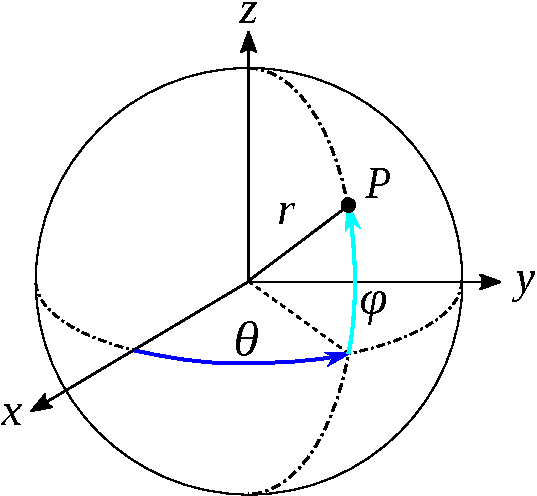
\includegraphics[width=0.35\linewidth]{../media/solidangle_cs.pdf}}
    \subfigure[Solid angle example graphic]{
        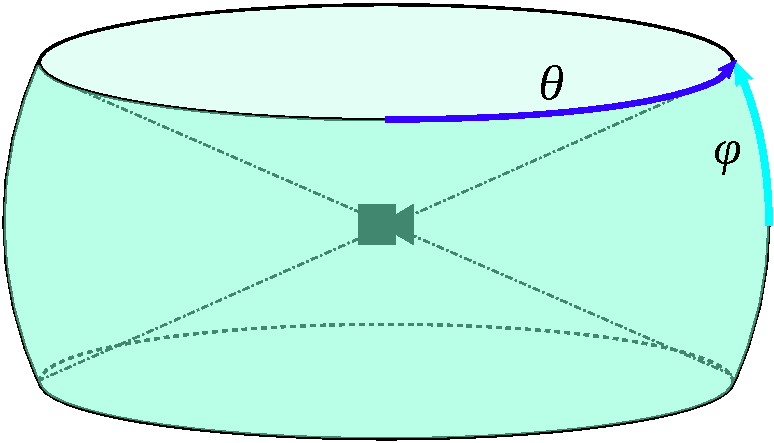
\includegraphics[width=0.5\linewidth]{../media/solidangle_ex.pdf}}
    \caption{(a) Spherical coordinate system for Equation \ref{eq_solidangle2}. (b) Example graphic demonstrating where angle values correspond to sensor. The transparent green region represents the sensor's visible field.}
    \label{solidangle}
\end{figure}

Given the information above, stereo sensors are the clear winner in terms of points per dollar (points/price) as well as point density (points/area).

On the question of quality, lidar becomes the de facto standard of measure due to its high accuracy.
This means that stereo vision quality is derived from how closely it matches a lidar scan. This also means that stereo vision quality is highly dependent on the system used, and can vary with both hardware and software implementation. A typical engineering threshold of 10\% is used for comparison, meaning that a single stereo-generated point is considered ``good" if its depth estimate is within $\pm$10\% of the absolute value of the corresponding lidar depth estimate. The horizontal and vertical distances, $x$ and $y$, are ignored due to the assumed 1:1 correspondence when projecting a point cloud onto the image plane. The steps to determine this quality are:

\begin{enumerate} \itemsep=-0.5em
    \item Project lidar points to image space, the resulting matrix named $L$
    \item Convert disparity values of stereo map to depth values, named $S$
    \item Keep only points from stereo map that also exist in $L$
    \item For each $(i=row,j=column)$ index, obtain the lidar distance, stereo distance, and the relative error between them as in Equation \ref{eq_errCalc} below.
    \item Tally how many points fall within the $\pm$ 10\% threshold as a percentage of the total points.
\end{enumerate}
\begin{equation}
    e = \left | \frac{S_{i,j} - L_{i,j}}{L_{i,j}} \right |
    \label{eq_errCalc}
\end{equation}

After performing the following steps, Figure \ref{corr_stereo_lidar} was generated: A lidar-stereo graph that merely indicates at what distance value a given stereo point has, and what value its corresponding lidar point also has.

\begin{figure}[ht]
	\centering
	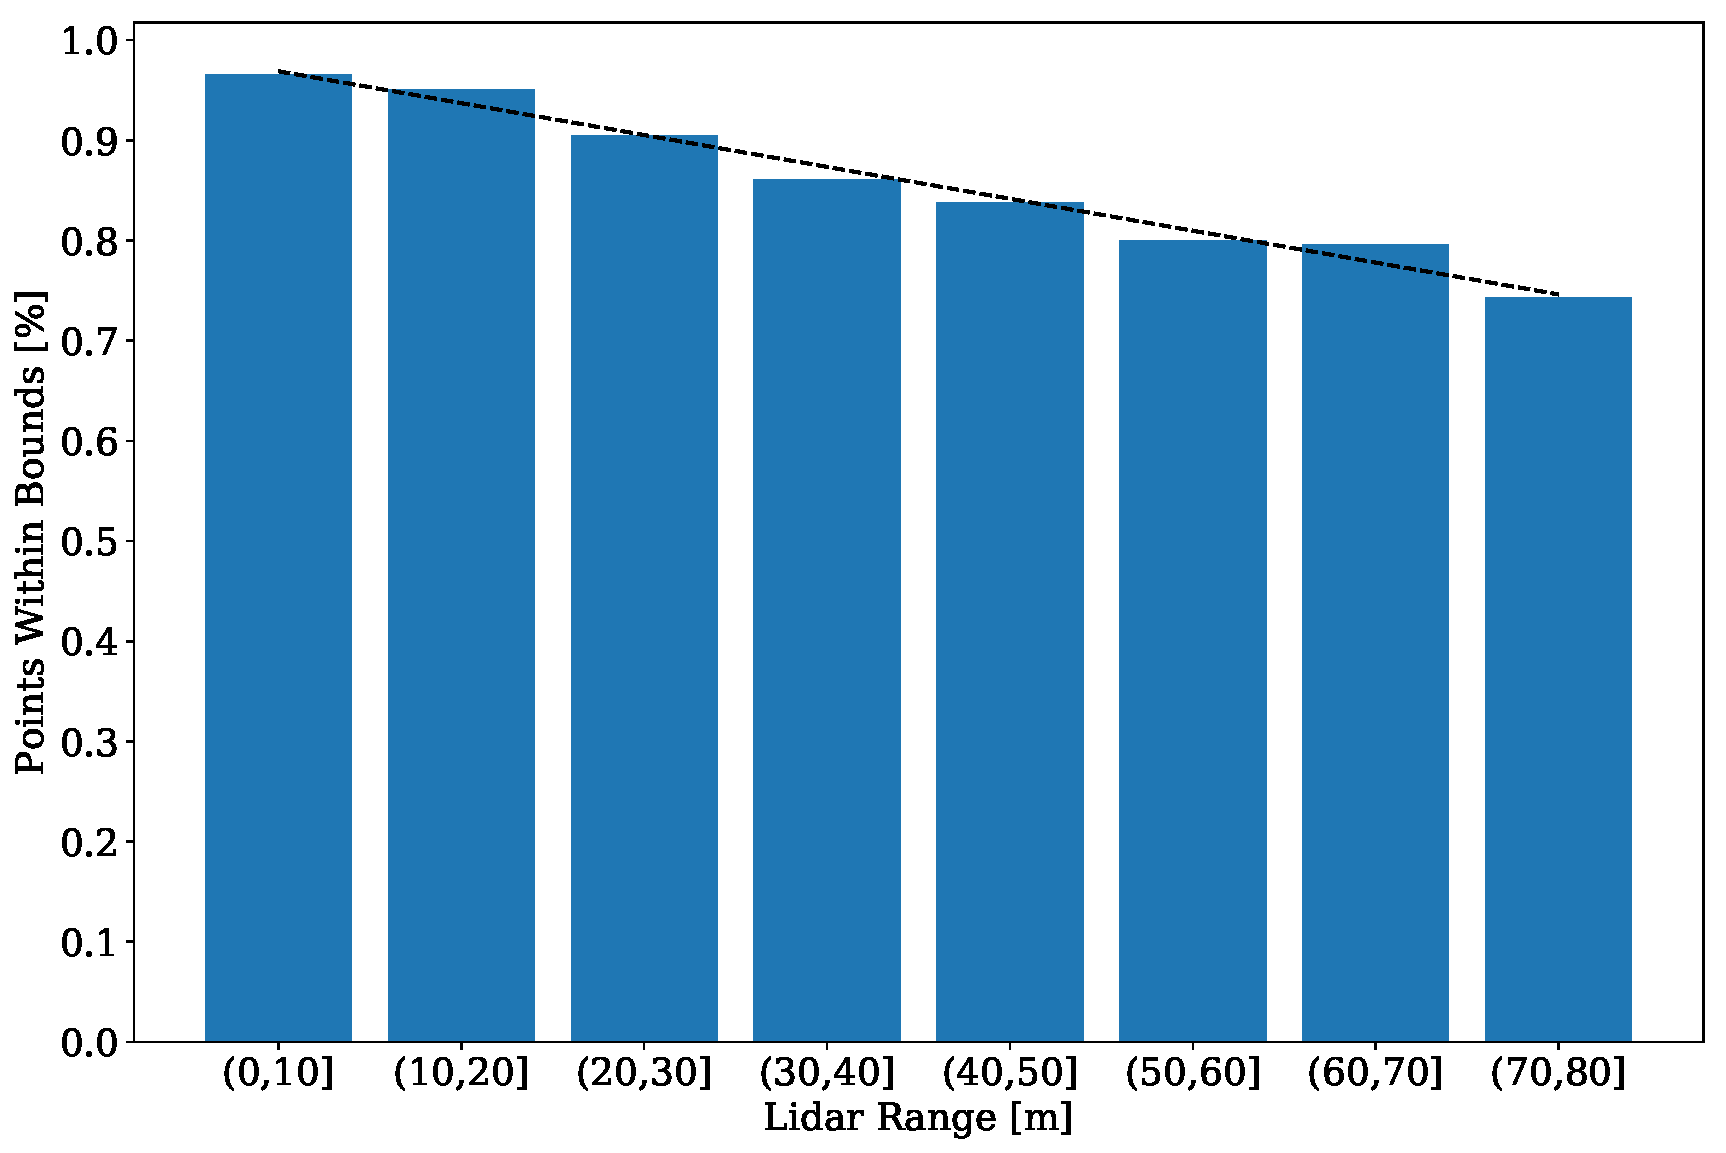
\includegraphics[width=0.8\linewidth]{../media/corr_pct_within.pdf}
	\caption{A bar chart describing what percentage of points lie within the given depth range. As an example, about 95\% of stereo depth values greater than 10 meters but less than or equal to 20 meters are within $\pm$10\% of the corresponding lidar depth value. The first 1000 indices of the KITTI dataset were used, altogether comprising 17,134,011 point comparisons between stereo and lidar. The dotted line indicates a 1st order polynomial fit, with the slope equal to about -0.03 percentage points per range (i.e. every 10 meters, there's about -0.03 change in percentage of points within bounds). In the smallest subset of points, the (70,80] range, there are 75,224 points.
	}
	\label{corr_stereo_lidar}
\end{figure}

In summary, stereo vision is an attractive alternative to lidar vision because of its much higher point density, lower price, reasonable quality approximation of lidar, and the potential to improve through further research. Under the correct conditions, stereo vision sensors have the potential to compete with lidar sensors in terms of both quantity and quality.



% NEWSECTION ===================================================================
\newpage
\subsection{Related Work} % status: stereo vision, 3D, etc

\subsubsection{Stereo Vision}
Stereo disparity maps are built by comparing the pixel distance between two similar regions of two images. Generating a disparity map, however, was developed before the popularization of neural networks. The key step that most neural networks have been used to improve is matching cost computation \cite{chang_pyramid_2018},  one of the four typical steps as described by Scharstein \cite{scharstein_taxonomy_2002}. Out of this paper, the four main parts of conducting stereo vision have been classically defined as follows: matching cost computation, cost (support) aggregation, disparity computation and optimization, and disparity refinement.

Initially, built-in and readily available stereo disparity map computation techniques were used. In the Python OpenCV library, there is a ``Semi-global Block Matching" (SGBM) algorithm, implemented based on the paper by \cite{hirschmuller_stereo_2007}. For an initial ``rough" pass, this algorithm was cheap and fairly effective. Additionally, this algorithm is useful for fast, fairly-stable calculations and does not need a GPU to run. However, it suffers from a few key shortcomings. For one, there is a large rectangular portion of the disparity map that contains no values, as can bee seen in the left side of Figure \ref{ind15_SGBM_comparison}(a), where missing values are marked red. Next, when a set of pixels cannot be matched between images, the result is simply a value of zero, giving no information in that region; these locations are also marked in red. Finally, SGBM suffers from a significant lack of resolution, meaning that some objects of interest, such as the three pedestrians in the image (highlighted with red rectangles in the color image), will not be seen well, or at all. For comparison, stereo images created with a neural network (NN) such as those in Figure \ref{new_psmnet} have a richer amount of information and have no missing pixels (i.e. a prediction is made at every pixel).

\begin{figure}[H]
    \centering
    \subfigure[SGBM disparity map]{
        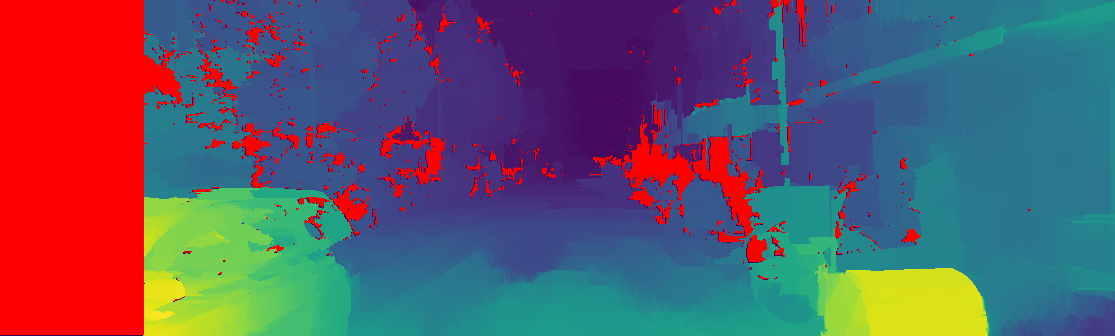
\includegraphics[width=1\linewidth]{../media/ind15_SGBM_comparison2.png}}
    \subfigure[LHS image]{
        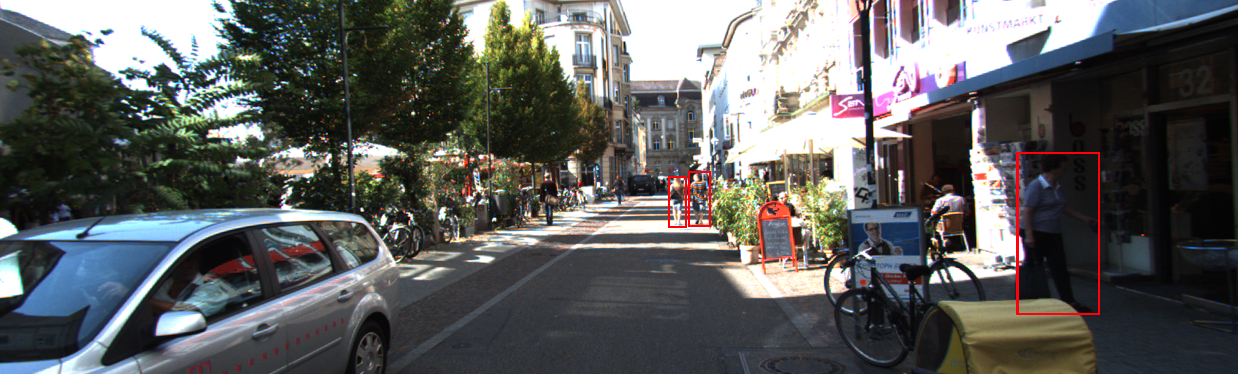
\includegraphics[width=1\linewidth]{../media/objdet_LHS_000015_withBox.png}}
    \caption{An example of a disparity map generated without a neural network approach. Though it has good merit, there are some noticeable shortcomings. This disparity map was generated in part by the left-side color image below. Index 15 of the KITTI Object Detection dataset.}
    \label{ind15_SGBM_comparison}
\end{figure}

With this knowledge, the next step was to find an ideal NN-based stereo disparity estimation method. Notable stereo neural network approaches to disparity estimation include Pyramid Stereo Matching network (PSMnet) \cite{chang_pyramid_2018} and iResNet \cite{liang_learning_2018}. In order to select the best candidate, multiple benchmarks were considered. The first benchmark was naturally the KITTI Stereo challenge, which contains a list of the top performing networks. At the start of this thesis writing, PSMnet stood in the top 10 of stereo networks in this list \cite{menze_kitti_2019}.

\subsubsection{3D estimation with Stereo Disparity Maps}
There is currently a low amount of public research on stereo vision for use with 3D localization. Most approaches are typically derived from a lidar-based approach. \cite{zeng2018rt3d} produced a stereo alternative to their original "Real-Time 3D Vehicle Detection" network, yet had a difficult time adjusting the performance to account for the noise present in a stereo-generated point cloud, as their approach first transformed points into a bird's eye view (BEV), then performed detections. This approach essentially works on a 2D image of the desired area, using well-established 2D localization methods, but from a top-down view. Also working in 2D, but with a more traditional approach, \cite{li_stereo_2019} takes the left and right images from each scene and obtains region proposals for both sides, eventually taking each proposal pair and estimating semantic information like ``object class, stereo bounding boxes, dimension", and so on. This approach does have its benefits, being deeply rooted in more traditional 2D localization techniques, such as those provided by \cite{ren_faster_2015}, but still experiences shortcomings due to working with three-dimensional data in a two-dimensional space. Additionally, some prior information is required, named as being a ``pre-set dimension prior" that is used for ``dimension prediction". In contrast, this paper and the state of the art approaches avoid the need to have prior information about the world. Overall, the network seemingly has some difficulty learning to estimate information in at least one of the dimensions. In contrast to these previous approaches, the state of the art is currently provided by \cite{wang_pseudo-lidar_2019} in an approach that reconstructs a stereo image into a point cloud, then manipulating the data in a three-dimensional space. Since the start of this paper, it became public knowledge, and was then published before this paper was completed. In their paper, ``Pseudo-LiDAR from Visual Depth Estimation", the authors took an extremely similar approach to this paper. Their network architecture takes a stereo image pair, generates a disparity map via Pyramid Stereo Matching network, converts it to a ``pseudo-lidar" scan, and extracts 3D bounding box estimations via Frustum Pointnet. This development unfortunately has a strong overlap with the contents of this paper, yet did not have origins in short-range detection of objects. However, in their paper, the authors argue that within a short distance, up to 30 meters away, stereo vision performs competitively with lidar, which is encouraging for the work performed here.

\subsubsection{3D Estimation with Lidar}
Performing 3D estimation and localization with lidar has been a focus for a large portion of the field, and with good reason. Lidar data, while expensive to obtain, currently provides the best option for 3D information. Thus, there are many papers which focus on using lidar sensor capabilities to estimate 3D bounding boxes, to varying degrees of success. As mentioned previously, \cite{zeng2018rt3d} attempted to use lidar information with a novel 2D BEV approach, yet fell short of really taking advantage of the new dimension that lidar provided. The greatest breakthroughs have indeed been by networks that manipulate the information directly in the 3D space. Notably, Volumetric CNN's such as by \cite{wu20153d} were one of the first leaps from 2D space to 3D space, using voxels created by the 3D information provided. However, this approach ultimately struggles with data sparsity and the massive computational cost of 3D convolution. Similar to the first two approaches named, multi-view CNN's such as that by \cite{su2015multi} attempt to use multiple 2D projections of the 3D space to estimate object locations. These also fail, namely when attempting to perform finer operations such as shape classification. One of the major successes in 3D object detection has been by \cite{qi_pointnet:_2017} in the development of Pointnets, a network that could directly and scalably ``summarize an input point cloud by a sparse set of key points". This had a built-in level of robustness, because the network was designed to operate on an orderless set of points, with less-than-complete knowledge of the 3D shape. However, an improvement came by the same authors when ``Frustum Pointnet", by \cite{qi_frustum_2017}, was introduced. This network simplified the classification process by first using a 2D object detector as a filter to isolate a region of the point cloud. This cone, or ``frustum", then allowed the Pointnet network to operate on a substantially smaller set of points, reducing computation time. This paper takes advantage of this capability to great effect.

% NEWSECTION ===================================================================
\newpage
\section{Pyramid Stereo Network and Disparity Map Reconstruction} % topic1
\label{sect_psmnet}
The network developed over the course of this thesis, called Stereo Point Cloud Network (SPCLnet) can be broken up into two main sub-networks, as shown below in Figure \ref{spcl_arch}. The first sub-network is explained here, and the second sub-network is explained in the next section.

\begin{figure}[ht]
	\centering
	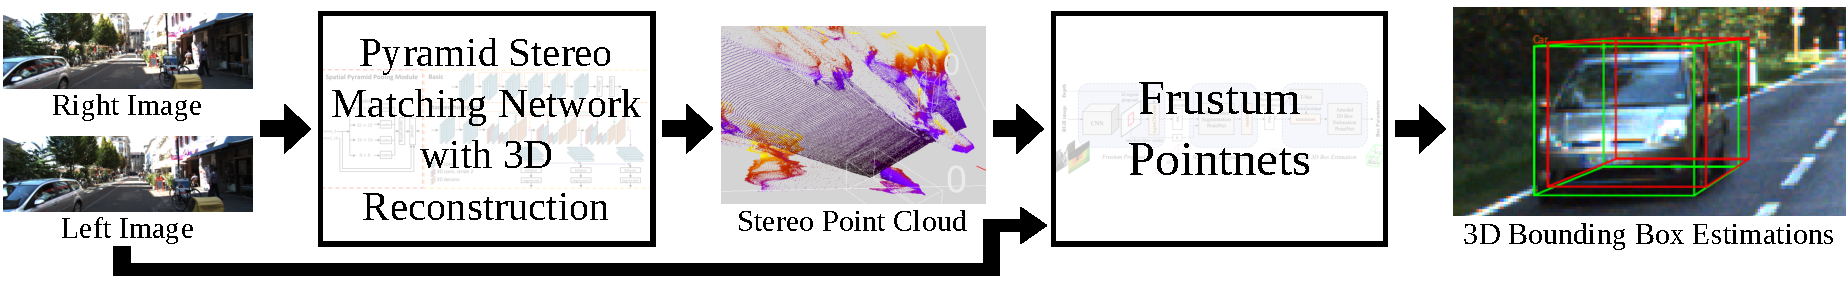
\includegraphics[width=1\linewidth]{../media/spcl_arch.pdf}
	\caption{General architecture of Stereo-Pointcloud network. A stereo image pair is fed to a disparity estimation network, specifically PSMnet, which then also reconstructs the disparity map into a 3D point cloud. The point cloud is then fed into a pointnet (along with the original left image), specifically Frustum Pointnet, which finally returns a 3D bounding box estimation. Images reproduced from \cite{geiger_are_2012}, \cite{chang_pyramid_2018}, and \cite{qi_frustum_2017}.}
	\label{spcl_arch}
\end{figure}

The first sub-network is used to generate a stereo-based point cloud from a disparity map estimation network, created by \cite{chang_pyramid_2018}. The majority of the following information is derived from their work. This sub-network consists primarily of a "Spatial Pyramid Pooling module" to look for matching information at various levels of detail, as well as a "stacked hourglass module for cost volume regularization". After the sub-network is described, a brief explanation of reconstruction is also provided. 

\subsection{Pyramid Stereo Matching Network}
The first task in creating a network that can take a stereo image pair and generate 3D bounding boxes, as described in Figure \ref{spcl_arch} above, is to have the capability of taking a stereo image pair and creating a 2.5D disparity map. To that end, a best-in-class disparity generation algorithm was searched for and selected to be the Pyramid Stereo Matching Network (PSMnet). PSMnet was published by Jia-Ren Chang and Yong-Sheng Chen in March 2018. This network takes a deep learning approach to generating disparity maps from a pair of images. The network itself is near the top of the state of the art, and achieves this by the architecture of its network. The openly-available repository provided a foundation to start on towards making a compact, easy-to-use function.

First, the original evaluation code was tested out. Some modification and housekeeping had to be done to ensure that it was compatible with the local installation, as well as being adapted for use with Python 3. All deprecated functionality was manually removed.

Pyramid Stereo Matching Network, or PSMnet, is a network that takes advantage of an hourglass-shaped network. The result are very high quality, high resolution disparity maps. The network takes advantage of GPU processing power, depending on nVidia's GPU acceleration, similar to other networks. The network itself is written in PyTorch, a flexible and python-based network module. The use of PyTorch enabled fast, simplified debugging. PSMnet's architecture is shown below in Figure \ref{psmnet_arch}.


\begin{figure}[ht]
	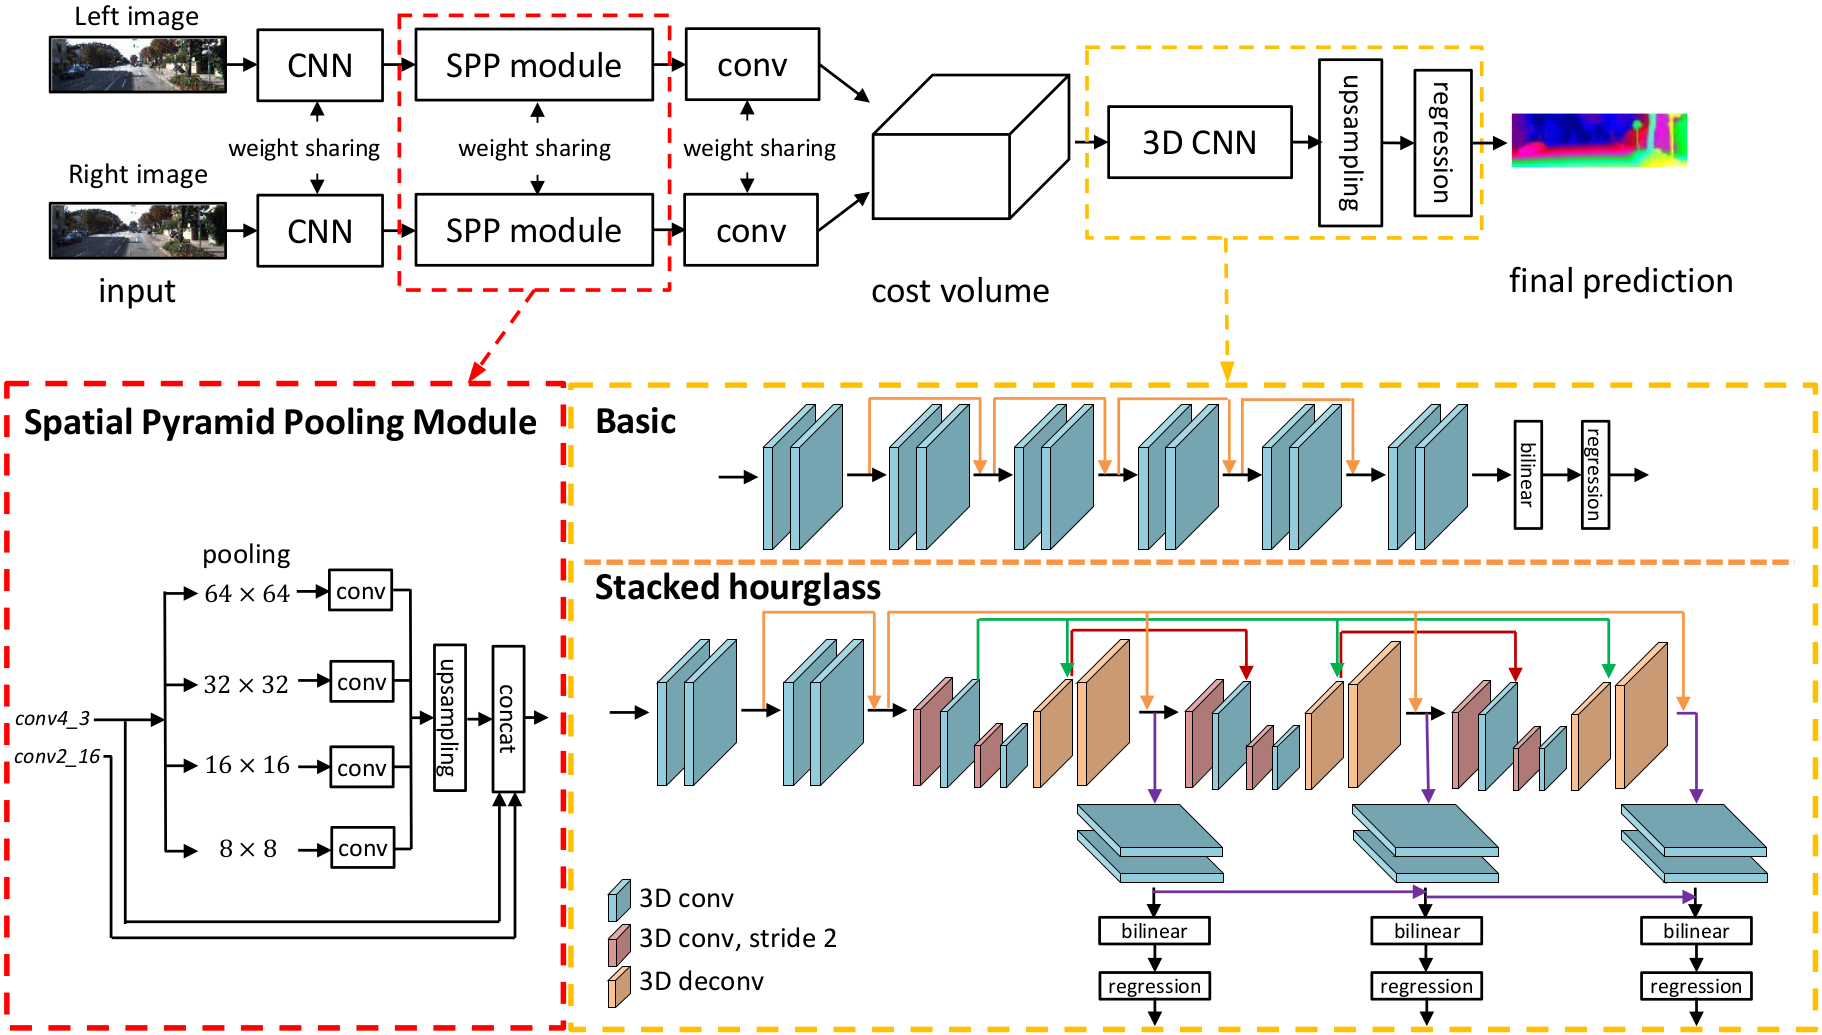
\includegraphics[width=1\textwidth]{../media/psmnet_arch.png}
	\caption{Generalized network architecture for Pyramid Stereo Matching network. The 3D CNN has two available configurations, Basic and Stacked hourglass. Stacked hourglass was used here. The Spatial Pyramid Pooling Module helps describe how features at varying ``zoom" levels were concatenated together. Image reproduced from \cite{chang_pyramid_2018}.}
	\label{psmnet_arch}
\end{figure}

\subsection{3D Reconstruction from Stereo Data}
\label{sect_reconstruct}
%things to cover: 
%1. introduction to reconstruction and methods
%2. where explained and referenced
%3. start with simple image describing the initial problem
%4. give equations, with explanation of variables
%5. give more concrete example of how one performs this, with both a disparity image and a given point cloud.
Reconstruction is the process of taking a series of 2D images and producing a 3D representation of that information \cite{szeliski_computer_2010}. In this project, reconstruction is a vital part of taking the disparity map estimation of one network and creating a pointcloud that is given to the second network. The main goal is to end up with a pointcloud, an unordered set of metric coordinates. Epipolar equations allow one to perform these conversions, which are explained below. The main sources for these equations come from both \cite{szeliski_computer_2010} as well as the mention of their usage in the paper by \cite{wang_pseudo-lidar_2019}. 

To begin describing how the transformation is done, a simple problem is presented with the following assumptions. Let there be two cameras in a scene, both facing the same direction and able to see an object at point $P$, such as a ball. The following assumptions are made: 

\begin{itemize} \itemsep=-0.5em
	\item The two cameras are identical in performance, producing equal quality images at the same point in time.
	\item The camera centers are aligned (for simplified rectification).
	\item Images produced are already rectified (to remove all distortion).
	\item The camera centers $O_i$ are separated by a baseline distance $b$.
	\item The two cameras have identical horizontal focal lengths $f_U$.
	\item The ball appears at some horizontal distance $x_i$, whether the origin is measured from the left side of the image or the center.
\end{itemize}

When the two cameras take an image of the ball, the light rays they capture may be drawn as given in Figure \ref{epipolar}. The figure gives a top-down view of what both cameras capture, and the horizontal pixel location at which the light ray comes into contact with each camera center. 

\begin{figure}[ht]
    \centering
	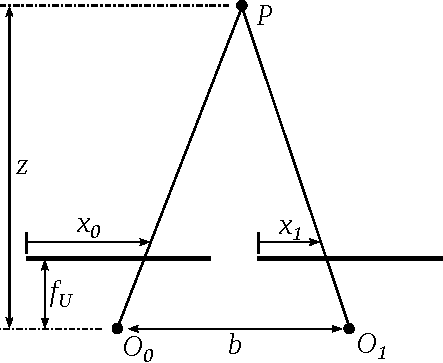
\includegraphics[width=0.4\textwidth]{../media/epipolar.pdf}
	\caption{Simplified graphic demonstrating how disparity may be derived from two cameras. The images the cameras produce must first be rectified and calibrated.}
	\label{epipolar}
\end{figure}

Given the above physical setup, the equation describing the relationship between disparity and depth $z$ may be found. When an entire array of disparity points is given, denoted as $D$, the resulting equation is then: 
\begin{equation}
z = \frac{f_U b}{D}
\label{eq_epi_z}
\end{equation}

For example, if the ball is located at 100 pixels away from the edge in the left image and 150 pixels away in the right image, then the disparity is 50 pixels. Thus, a disparity map may be generated by looking for matching features in two images and assigning each location a difference in the value of where one is found in reference to another (typically the left image is the reference).

The process of determining horizontal distance $x$ and vertical distance $y$ merely requires further application of the system in three dimensions rather than two, and may be calculated then as: 
\begin{equation}
x = \frac{z (u - c_U)}{f_U}
\end{equation}

\begin{equation}
y = \frac{z(v - c_V)}{f_V}
\end{equation}

It is important to note that $D$ stands for a disparity matrix, $f_U$ and $f_V$ are for horizontal and vertical focal lengths (respectively), ($c_U$,$c_V$) are the pixel center of the image, and $(u,v)$ represent a (column, row) coordinate location in $D$. 

In practice, the calculation is performed in a series of matrix calculations rather than as an element-by-element operation. These steps are covered below with accompanying Python code. This code assumes the usage of the Numpy module and that the disparity map has already been generated and saved.

The first step in the reconstruction process is determining the baseline $b$, horizontal focal length $f_U$, vertical focal length $f_V$, and image center $(C_U,C_V)$. The baseline is quickly obtained from KITTI development kit files, which list it as a fixed value of 0.54 meters. The accuracy of this measurement is not known beyond that. For each scene, the focal lengths are determined directly from the left color camera calibration matrix $P_2$, where $f_U=P_2[0,0]$ and $f_V=P_2[1,1]$. The image centers are found by dividing the disparity dimensions by half of the image dimensions, which corrects for non-standardized image dimensions present throughout the dataset. The depth array $Z$ is calculated via matrix operations in nearly the same way as given in Equation \ref{eq_epi_z}. All code used for both producing this work as well as the graphics can be found in the repository by \cite{gonzalez_smart3d_2019}. 

\begin{lstlisting}
import numpy as np
# STEP 1: generate / load a disparity map
disp=np.load(dpath)

# STEP 2: obtain parameters
P2 = rec.P2 # pre-existing object that parses calibration file
fHoriz = P2[0,0]
fVert= P2[1,1]
Baseline = 0.54 # meters. Obtained from devkit
imH,imW = np.array(pil.open(lpath).convert('RGB')).shape
Cu=disp.shape[1]-imW/2 # Cu = imW/2 - (imW - dispW)
Cv=disp.shape[0]-imH/2 # Cv = imH/2 - (imH - dispH)

# STEP 3: Calculate depth from disparity values
zvals = fHoriz*baseline/disp
\end{lstlisting}

Once this has been performed, the $X$ and $Y$ matrices are generated by creating a vectorized forms of their corresponding theoretical equations: 
\begin{lstlisting}
# STEP 4: Convert x_px & y_px to metric
xpos=np.arange(0,zvals.shape[1])-Cu
ypos=np.arange(0,zvals.shape[0])-Cv
ulocs=np.tile(xpos*-1,(zvals.shape[0],1))
vlocs=np.tile(ypos*-1,(zvals.shape[1],1)).T
xvals = ulocs*zvals/fHoriz
yvals = vlocs*zvals/fVert
\end{lstlisting}

Once each matrix has been created, they may be combined to form a vector of three dimensional coordinates, as shown below in Figure \ref{reconstruction}(e). 

\begin{figure}[H]
    \centering
    \subfigure[left image]{
        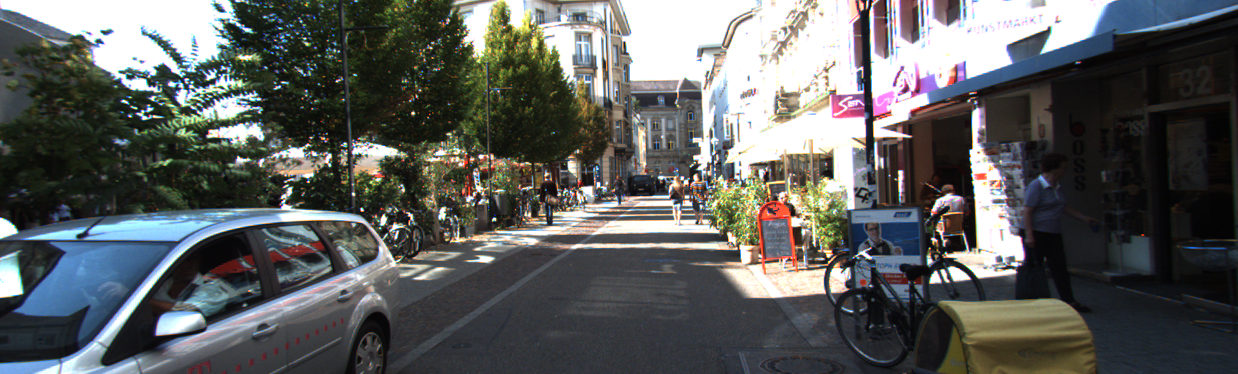
\includegraphics[width=0.487\linewidth]{../media/objdet_LHS_000015.png}}
    \subfigure[right image]{
        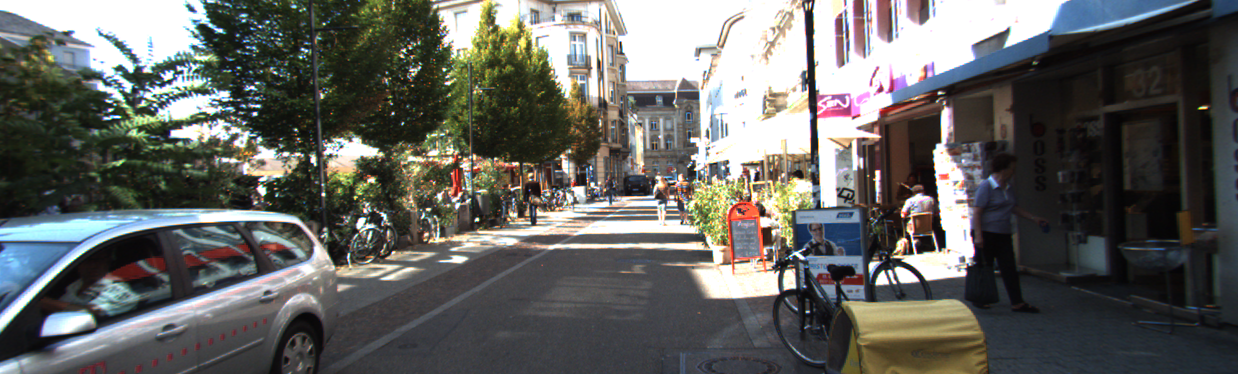
\includegraphics[width=0.487\linewidth]{../media/objdet_RHS_000015.png}}
    \subfigure[disparity map]{
        
\includegraphics[width=0.487\linewidth]{../media/ind15_psmstar_v190613_AsOf190626.png}}
    \subfigure[depth map]{
        
\includegraphics[width=0.487\linewidth]{../media/ind15_disp2depth.png}}
    \subfigure[final point cloud result]{
        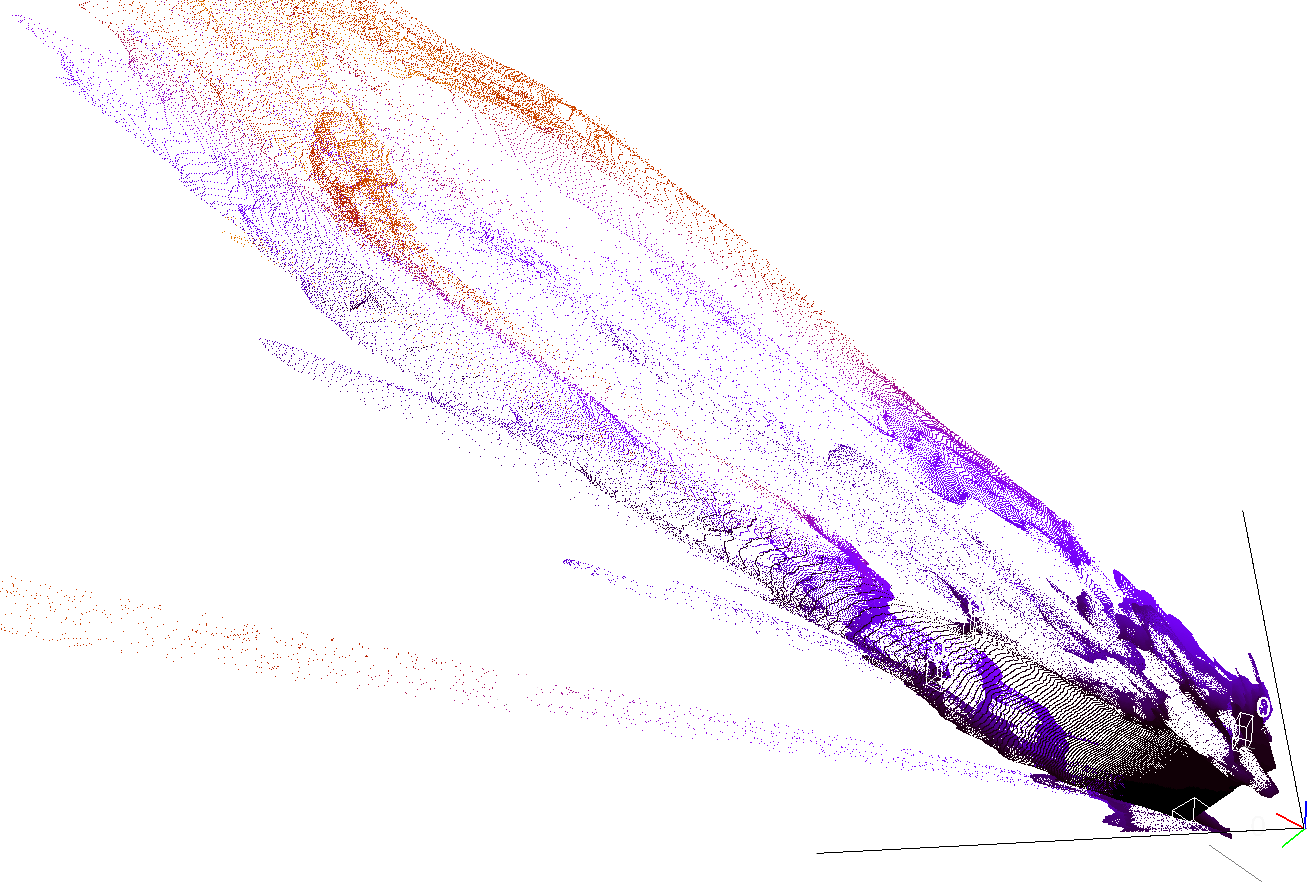
\includegraphics[width=\linewidth]{../media/ind15_disp2pcl.png}}
    \caption{Various states of transformation from an image pair to a point cloud. Two images, (a) and (b) are given to PSMnet, which outputs a disparity map (c), which is changed to a depth map (d) via \ref{eq_epi_z}, and is finally transformed into a point cloud (e) with the remaining two epipolar equations. Subfigure (e) shows the camera horizontal field of view with two black lines.}
    \label{reconstruction}
\end{figure}






% NEWSECTION ===================================================================
\newpage
\section{Point Clouds and Frustum Pointnet} % topic2
\label{sect_fpnet}
\subsection{Development of Stereo 3D Reconstruction Function}
As described in Section \ref{sect_reconstruct}, the overall steps of reconstructing the resulting stereo image consisted of three general equations adapted for use with matrix operations. This also included selecting the proper constants for each calculation. To achieve all this, a specific class was created that would initialize by loading the fully trained model and use it in a non-learning ``testing" mode, whereby it would take in either an image path pair or a loaded pair of image arrays. The pair would then be evaluated in PSMnet, which returns a stereo map, and finally be converted to a pointcloud using the epipolar equations in matrix form. Each record of the KITTI dataset has its own calibration file, but the baseline value remained the same. During the overall Frustum Pointnet training and evaluation, a new pointcloud would be generated in real-time.

\subsection{Modification of Frustum Point Net}
Frustum Pointnet, being originally written for Python 2, needed to undergo some minor adaptations while being modified for usage with Python 3. For example, several modules and functions were deprecated or needed modification, and so had to be properly adapted. There are also two actively maintained versions of the frustum Pointnet code. as explained in the original paper \cite{qi_frustum_2017}, there are two versions of the FPNet model: the first which uses standard Tensorflow libraries, and the second which uses custom Tensorflow operators that must be compiled. For the purposes of this paper, version 1 was used and will be the default version unless otherwise noted.

In order to transition from using the provided pre-trained model and preprocessed data to self-made preprocessed and trained data, a set of steps and ``paths" were created to guide what was happening in each step and set of ``runs". As shown below in Figure \ref{fp_paths}, there are various steps with gradually increasing dependence on stereo-based pointcloud data.

\begin{figure}[H]
    \centering
    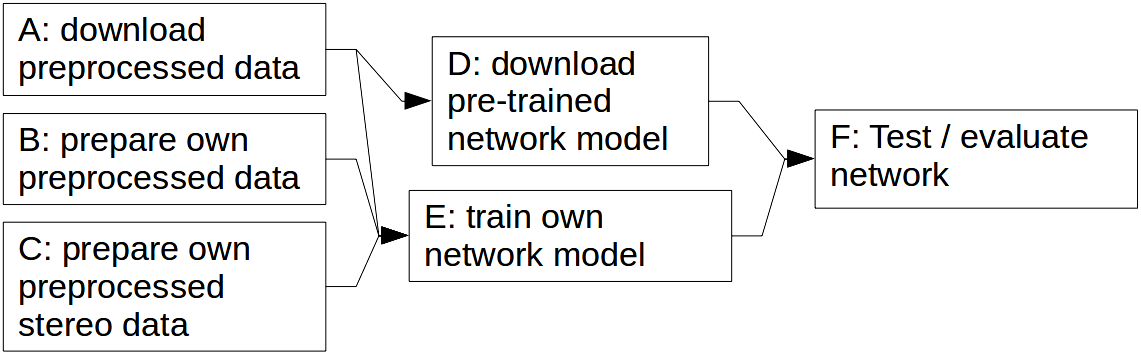
\includegraphics[width=1\textwidth]{../media/fpnet_paths_img.png}
    \caption{Various paths that were planned to simply transition from lidar-based 3D estimation to stereo-based 3D estimation. Generally, paths went chronologically as follow: ADF, AEF, BEF, and finally CEF.}
    \label{fp_paths}
\end{figure}

The most basic path, ADF, is simply using the given model to evaluate and achieve similar results to the official paper. Next, AEF used lidar pointclouds, but the model was trained locally. BEF required locally running the ``preprocessing" step, but was still theoretically identical to the previous two paths. Finally, CEF truly deviates from the other paths by using a stereo-generated pointcloud to preprocess data, then train on that, and finally evaluate the model's detection capability.

The general architecture of FPnet is described below in Figure \ref{fpnet_arch}, reproduced from the original paper by \cite{qi_frustum_2017}. 

\begin{figure}[H]
    \centering
    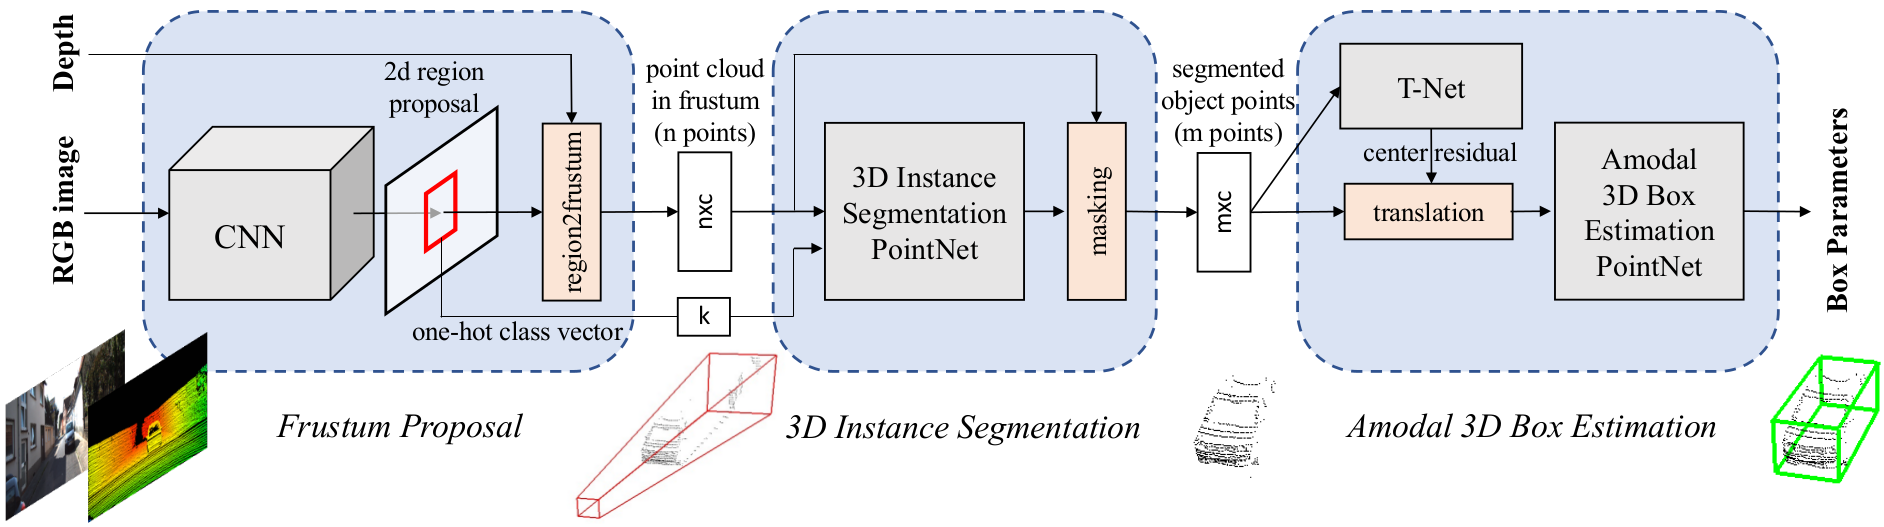
\includegraphics[width=1\textwidth]{../media/fpnet_arch.png}
    \caption{Frustum Pointnet architecture. Reproduced from paper by \cite{qi_frustum_2017}.}
    \label{fpnet_arch}
\end{figure}

The network itself works in three separate but closely related steps: 
\begin{enumerate}
    \item Frustum Proposal: A 2D CNN takes an RGB image and localizes a set of detections as region proposals, also generating a "one-hot" class vector that determines which classes are searched for in the next step.
    \item 3D Instance Segmentation: For each region proposal, a cone or ``frustum" is cut out from the point cloud, a and a 3D instance segmentation is performed, and a masking step removes both needless foreground and background points.
    \item Amodal 3D Box Estimation: Each filtered subset of the point cloud is then subjected to amodal 3D box estimation, meaning that the incomplete set of points are then used to estimate a final set of 3D bounds defining the estimate for each detection.
\end{enumerate}







% NEWSECTION ===================================================================
\newpage
\section{Experiments}
\label{sect_experiments}
Once the network was built and implemented, several experiments were conducted and iterated upon in order to achieve the best possible performance with the given datasets and knowledge. The first subsection is dedicated to explaining the performance metrics of 3D object detection, then moves on to describing the results of each experiment and investigation performed with the network. As noted below and in the results of each experiment, the class "Car" is the sole class that is examined. Other classes, such as Cyclist and Pedestrian, have evaluation code and even good ground truth labeling for them, but not in the sheer volume that the Car class has. See Appendix \ref{appendix_kitti} for more information. All code used in both producing the results as well as the graphics of this paper are provided by \cite{gonzalez_smart3d_2019}. 

\subsection{Performance Metrics}
In order to determine the quality of results obtained, a few different metrics are implemented as are standard in practice. Here, the various metrics are explained, and in Appendix \ref{appendix_metrics} examples are provided. The concept of verifying accuracy in a statistical estimate is covered in \cite{manning_introduction_2008}, and some of this information is covered briefly below. In the field of image recognition, one particularly interesting metric is ``Intersection over Union", also referred to as IOU or Jaccard Index. From this metric, precision and recall may then be calculated. Precision and recall are fundamental in obtaining more abstracted metrics such as average precision (AP) and mean average precision (mAP), which are how different networks are compared. The following information is primarily taken from the well-known PASCAL VOC (visual objects classes) Challenge \cite{everingham_pascal_2010} and ``An Introduction to Information Retrieval" by \cite{manning_introduction_2008}.

\subsubsection{Defining an Outcome}
The first step in measuring performance is categorizing what a result may be. With a visual task such as object classification, there are 4 possible outcomes (all references to true/false positive/negatives in this document will be referred to as ``outcomes"), which will be  as shown below. In general, there may be a True Positive, False Positive, True Negative, or False Negative outcome. In practice, True Negatives are not used, and the remaining three are used to varying degrees. Each is better clarified as such:
\begin{itemize} \itemsep=-.5em
	\item True Positive: Correctly detecting a true object
	\item False Positive: Incorrectly detecting something that isn't there
	\item False Negative: Incorrectly ignoring a true object
	\item True Negative: Correctly ignoring something that isn't there
\end{itemize}

\begin{figure}[H]
	\centering
	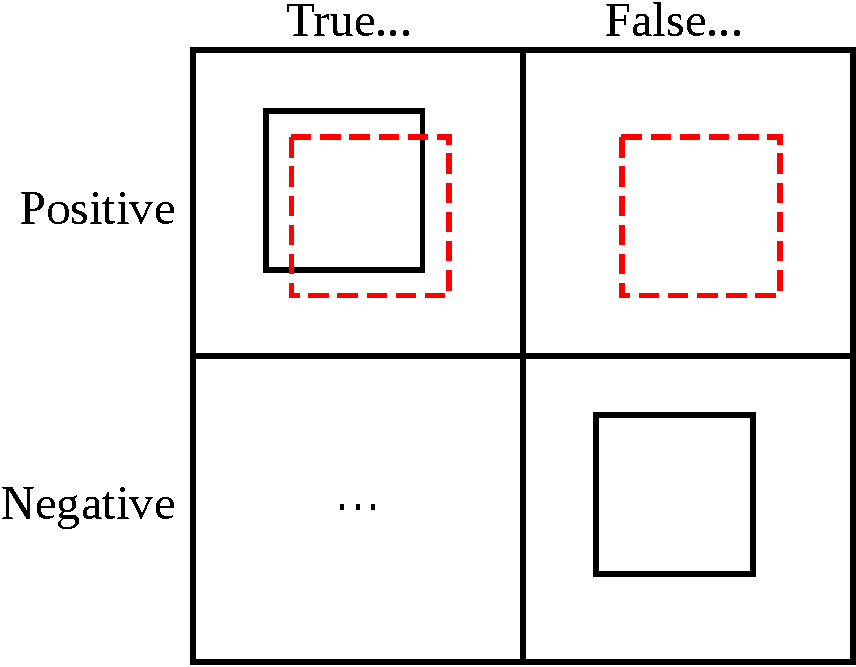
\includegraphics[width=.3\textwidth]{../media/tp_help.pdf}
	\caption{A visual representation of various outcomes, ground truths as solid black boxes and detections as dotted red boxes.}
	\label{tp_help}
\end{figure}

To actually classify a result in one of these categories, computer vision depends on using the overlap of a given bounding box estimate with a bounding box ground truth. If the overlap is above some threshold, the estimate is said to be a true positive. In some metrics, two estimates overlapping the same ground truth will only count the larger overlap, or the more confident estimate. This overlap is formally known as an Intersection over Union (IOU) value, or a Jaccard index.

\subsubsection{Intersection Over Union}
In image recognition, as well as other spatially-based tasks, accuracy is needed in various forms to know ``how well" a prediction overlaps, or matches, the ground truth. If, for example, an object-detection algorithm predicts the location of a car in a photo, one would like to know if such an estimate has any value, ideally with as few parameters as possible.

In light of this, IOU encompasses all relevant aspects of rating the overlap of two geometric shapes (e.g. rectangles) while enabling an intuitive, non-binary scoring of an estimate. IOU is calculated as two bounding regions' intersection over their union, just as the name states. Visually, this looks something like the below in Figure \ref{iou_img}. Uniquely, the calculation of area and intersection specifically for image boundaries is inclusive of the bounds, meaning that the length of a given difference must have ``+1" added to it.

In order to formally calculate IOU, a generalized form may be generated to apply to n-dimensions. The generalized mathematical equation is simply as follows. Given a region A and a region B:
\begin{equation}
IOU = \frac{|A\cap B|}{|A\cup B|} = \frac{|A\cap B|}{|A|+|B|- |A\cap B|}
\end{equation}

\begin{figure}[ht]
    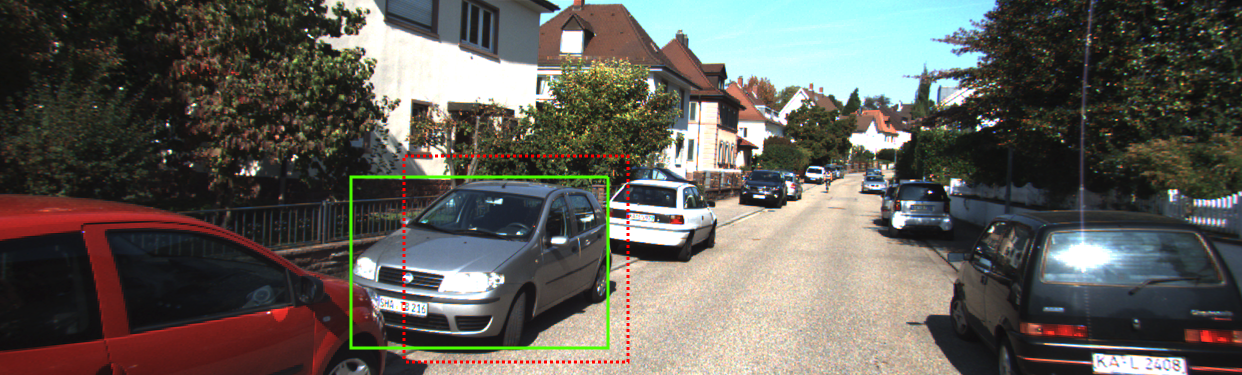
\includegraphics[width=1\textwidth]{../media/iou_img.png}
    \caption{Example of ground truth bounding box (solid green) and prediction bounding box (dashed red). In this image, the overlap between the green and red regions is the intersection, while the combined area is the union. The IOU of the two boxes is 0.64. Index 8 of the KITTI Object Detection dataset.}
    \label{iou_img}
\end{figure}

\subsubsection{Precision \& Recall}
\label{subsect_precrec}
Once all detections have been tallied and placed into their correct categories, their precision and recall may be calculated. In information retrieval, precision is defined as ``the fraction of retrieved documents that are relevant", and recall is defined as ``the fraction of relevant documents that are retrieved". Reworded for object detection: precision is the number of correct predictions divided by the total number of predictions, and recall is the number of correct predictions divided by the total number of possible answers. These two are also given as equations in terms of true positives and so on.

\begin{equation}
Precision = \frac{TruePositives}{TruePositives + FalsePositives}
\label{eq_prec}
\end{equation}

\begin{equation}
Recall = \frac{TruePositives}{TruePositives + FalseNegatives}
\label{eq_rec}
\end{equation}

Theoretically, precision and recall are generated at multiple points by varying a probability threshold and graphing each result. In practice, a precision-recall curve is generated by a more complex process that involves taking the cumulative sum of the detections in order of descending confidence level (1.0,0.99, ...). Once a precision vector and a recall vector have been created, the plot may appear something like below, reproduced from Figure \ref{precrec_steps} in Appendix \ref{appendix_metrics}. 

\begin{figure}[H]
	\centering
	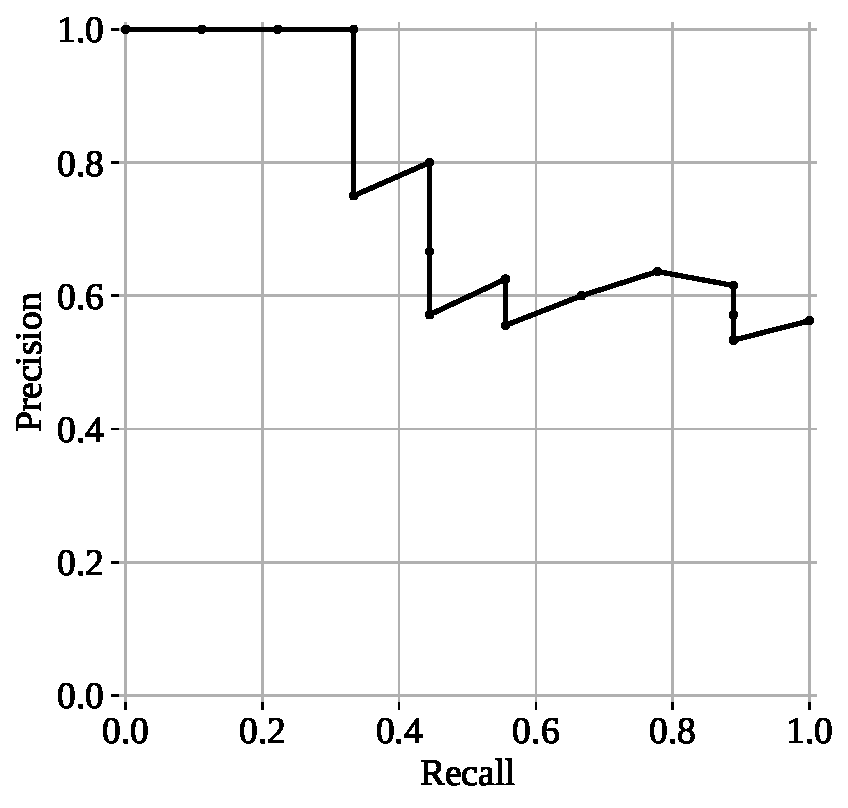
\includegraphics[width=0.4\linewidth]{../media/precrec_steps.pdf}
	\caption{A typical precision-recall curve. Taken from the example in Appendix \ref{appendix_metrics}.}
\end{figure}


\subsubsection{Calculating Average Precision}
Once a set of recall and precision data has been calculated, then AP is a fast and simple calculation. Formally, average precision is defined as the area beneath a precision-recall curve. However, this metric has been calculated in various forms and often modified by the scientific community, including the previously common 11-point average precision used by the Visual Objects Challenge (VOC), used until 2009 and by several subsequent object recognition challenges. 11-point AP has been argued to be slightly more robust against very jittery curves, but also judges results rather ``crudely" and less accurately \cite{everingham_pascal_2015}. For the purposes of computer vision, AP may also be considered a weighted sum of precision, considering that the differences in recall value may be used as the weights since their sum is 1. Thus, to match the function output by \cite{pedregosa_scikit-learn:_2011}, one may simply take a rectangular numerical integration of the values in Table \ref{precrec_ans}. It must be kept in mind that the order of the values MUST be in order of ascending recall value. The mathematical formula for calculating AP is then given in \ref{eq_ap}, where 1 is the starting index and $n$ is the length of the vector:

\begin{equation}
AP = \sum^{n-1}_{i=1} ({re}_{i+1}-{re}_{i})({pr}_{i+1})
\label{eq_ap}
\end{equation}

\subsection{Experiment 1: Lidar-Based Performance as a Baseline}

To first properly understand the performance capability of lidar-based 3D object detection, the typical pipeline was first verified locally. There are multiple setup steps as given by the authors, with a specific training-validation split. This was followed, and the performance was indeed on par with what exists officially on the KITTI 3D Object Detection benchmark. As described in Figure \ref{fp_paths}, there are three paths that emulate the methodology official results, all of which use lidar as the source of point cloud information: 

\begin{itemize} \itemsep=-0.5em
	\item ADF (downloading the pretrained model and evaluating immediately)
	\item AEF (download preprocessed data, train network, and evaluate)
	\item BEF (prepare preprocessed data, train network, and evaluate)
\end{itemize}

Aside from path ADF, which of course features no training component, the training loss of each path is visualized below in Figure \ref{fpnet_loss1}. path "AEF" was performed twice (revision 0 and revision 1), during different times in the project; The performance remained relatively consistent, however.

\begin{figure}[H]
	\centering
	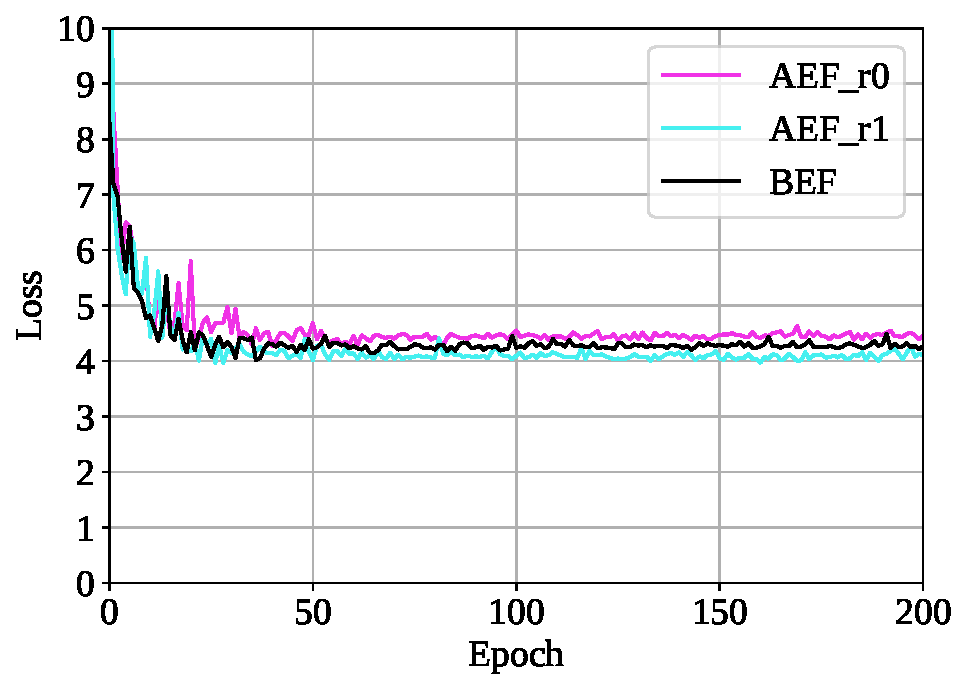
\includegraphics[width=0.6\linewidth]{../media/fpnet_loss1.pdf}
	\caption{Loss over epochs graph for Experiment 1. Run AEF\_r1 achieved the lowest training loss, settling to a value of around 4.1. The loss value represents an average score of how much a network predicts incorrectly during training.}
	\label{fpnet_loss1}
\end{figure}

Taking a slightly closer look at the training data, the lowest value loss that the network achieved while training was 4,1. The rate at which loss was changing also seemed to decrease to zero, indicating that the network was quite stable in its weights by the end of the training. For future reference, path BEF will be used to compare to other networks since it performed reasonably "average".

Additionally, the precision-recall curve of each path for the ``Car" class is also shown in Figure \ref{fpnet_pr1}. The curves generally indicate that the lidar-based point clouds were quite robust, and the AP score for the three paths are as follow.

\begin{table}[ht]
	\centering
	\caption{FPNet lidar-based results, across varying difficulties. BEF performed marginally better than the other runs, and was thus used as a reference in future experiments. AP score is calculated by finding the area under the precision-recall curve.}
	\begin{tabular}{|c|c|c|c|}
		\hline
		\b{Path} & \b{AP\_Easy} & \b{AP\_Med} & \b{AP\_Hard} \\ \hline
		  ADF    &    84.07     &    71.28    &    63.35     \\ \hline
		  AEF0   &    82.59     &    68.72    &    61.25     \\ \hline
		  AEF1   &    83.51     &    68.99    &    61.04     \\ \hline
		  BEF    &    84.12     &    71.00    &    63.27     \\ \hline
	\end{tabular}
	\label{fpnet_ap1}
\end{table}


\begin{figure}[H]
	\centering
	\subfigure[]{
	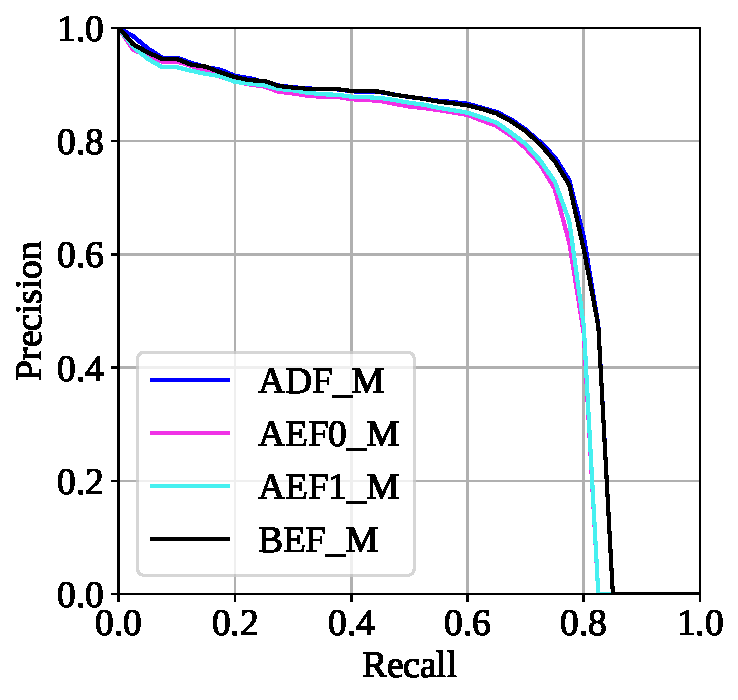
\includegraphics[width=0.4\linewidth]{../media/fpnet_pr1_multi.pdf}}
	\subfigure[]{
	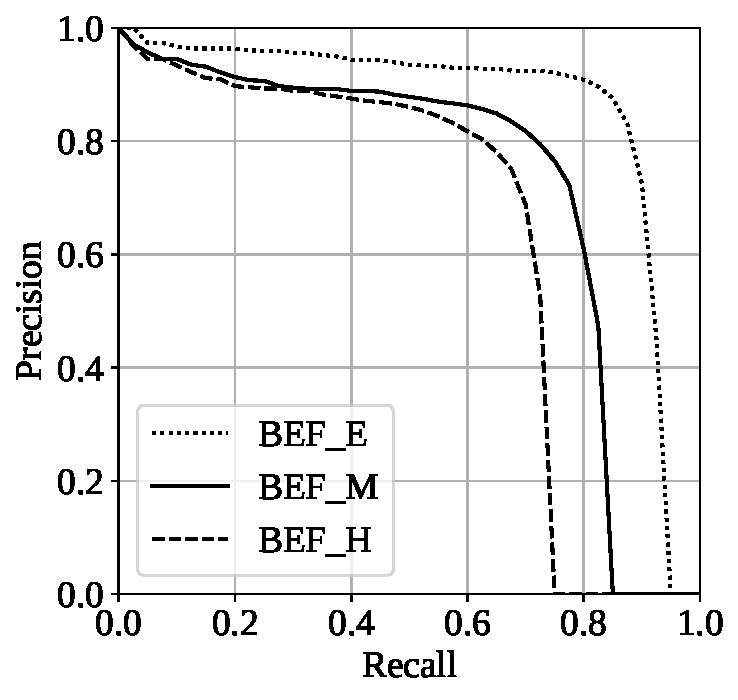
\includegraphics[width=0.4\linewidth]{../media/fpnet_pr1_bef.pdf}}
	\caption{Precision recall curves for Experiment 1. Subfigure (a) shows various runs at compared medium difficulty, while Subfigure (b) shows the best-performing run BEF at Easy, Moderate, and Hard difficulties.}
	\label{fpnet_pr1}
\end{figure}




Given that these are results from a lidar-based network, they are therefore the benchmark against which performance was then measured. 

\subsection{Experiment 2: Stereo-Based Performance, using Stereo Dataset}
The first experiment had the objective of using the stereo network, once trained, to provide a new source of point cloud data. This experiment corresponds with the path ``CEF": preparing preprocessed data with stereo vision instead of lidar, train the network model on this information, then evaluate the network performance. Because this experiment was later further modified, it is known as CEF\_r0, while the second version is named CEF\_r1. 


The training loss is provided below in Figure \ref{fpnet_loss2}, with a comparison to previous the previous, lidar-based path ``BEF". 

\begin{figure}[ht]
	\centering
	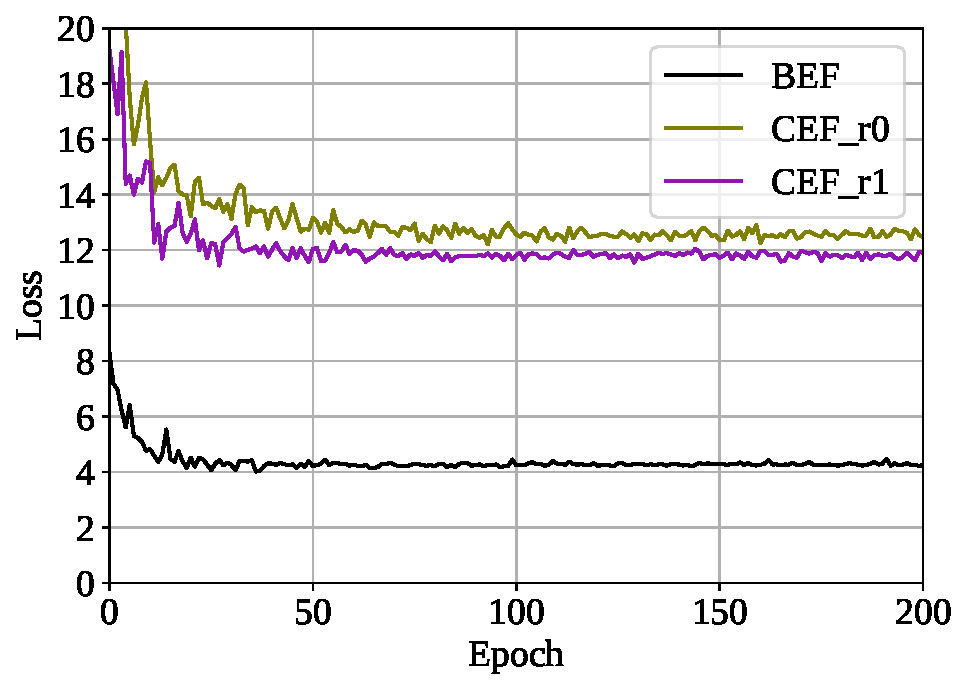
\includegraphics[width=0.6\linewidth]{../media/fpnet_loss2.pdf}
	\caption{Loss over epochs graph for Experiment 2. Run CEF\_r1 achieved the lowest final loss value, although reference curve BEF shows that lidar-based methods typically achieve lower loss during training.}
	\label{fpnet_loss2}
\end{figure}

As can be seen from the figure, the training loss also reached a point of equilibrium and ceased decreasing after some time, but at a much higher value than path BEF. CEF\_r0's loss value instead settled closer to a value of 12.4. 

In the evaluation, CEF\_r0 performed at a significantly lower level than BEF, indicating a need to further refine the model. However, there is some promise in this result, as it indicates that the system does perform well in the ``Easy" mode, when cars are generally within 30 meters of the sensor. The results from this experiment, as well as further reading, motivated the next experiment conducted. This is shown below, in Figure \ref{fpnet_pr2}.

After the initial results CEF\_r0, the 3D reconstruction step was reexamined for any possible errors. It was then discovered that PSMnet internally crops stereo image pairs into a standardized size, a significant piece of previously unmentioned information. The primary cause of non-standardized image sizes in the object detection dataset is due to the rectification performed on each raw image. This means that the images, after being rectified, are then cropped in a non-standardized way to remove the resulting non-image regions. PSMnet itself only works on a standardized image size, so it therefore takes the smallest dimensions across the dataset and crops all image pairs to that size, [1232,368] pixels. The PSMnet crop is anchored at the bottom-right corner of each image, which provides some consistency but may still contribute to a source of error, since the exact method of cropping both rectified data and images for stereo processing are not totally aligned. A second and lesser source of possible error that was corrected in CEF\_r1 was the method of reconstruction used. This updated method is reflected in \ref{sect_reconstruct}. The constant being used for all disparity-to-depth transformations was consistent, rather than being the product of baseline and $F_U$, horizontal focus length. Thus, Figure \ref{fpnet_pr2} and Table \ref{fpnet_ap2} show the improvement from CEF\_r0 to CEF\_r1. 

\begin{table}[ht]
	\centering
	\caption{Experiment 2 results, with Frustum Pointnets using stereo data. Average precision shown for the first two attempts, across varying difficulties, for the Car class.}
	\begin{tabular}{|c|c|c|c|}
		\hline
		\b{Path} & \b{AP\_Easy} & \b{AP\_Med} & \b{AP\_Hard} \\ \hline
		CEF0   &    35.61     &    23.02    &    20.43     \\ \hline
		CEF1   &    42.57     &    28.60    &    24.07     \\ \hline
	\end{tabular}
	\label{fpnet_ap2}
\end{table}

\begin{figure}[H]
	\centering
	\subfigure[]{
		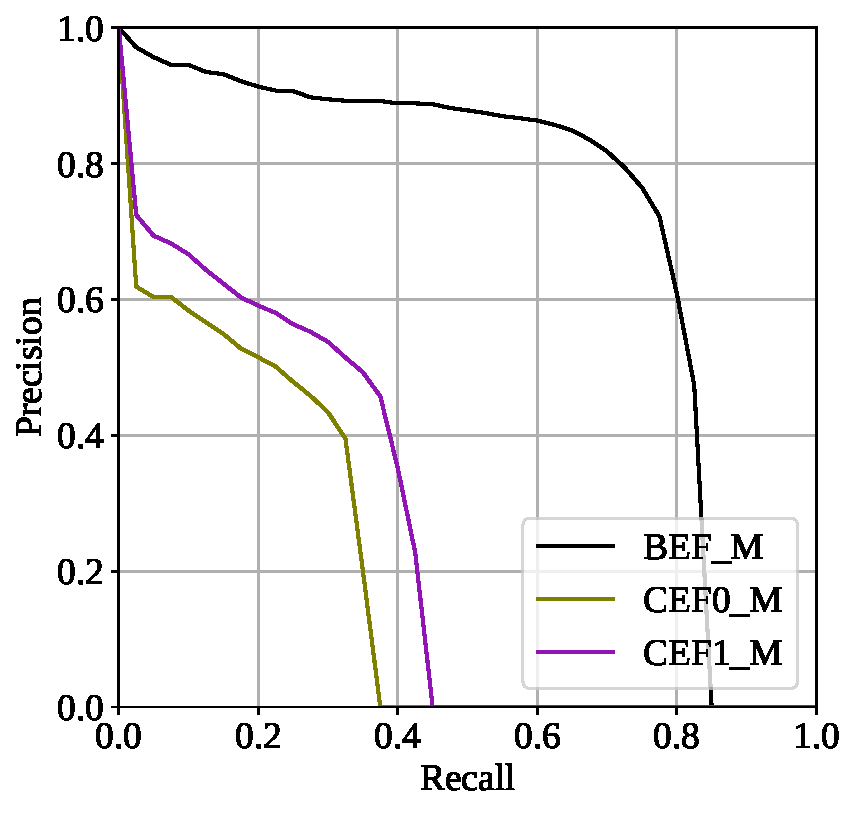
\includegraphics[width=0.4\linewidth]{../media/fpnet_pr2_multi.pdf}}
	\subfigure[]{
		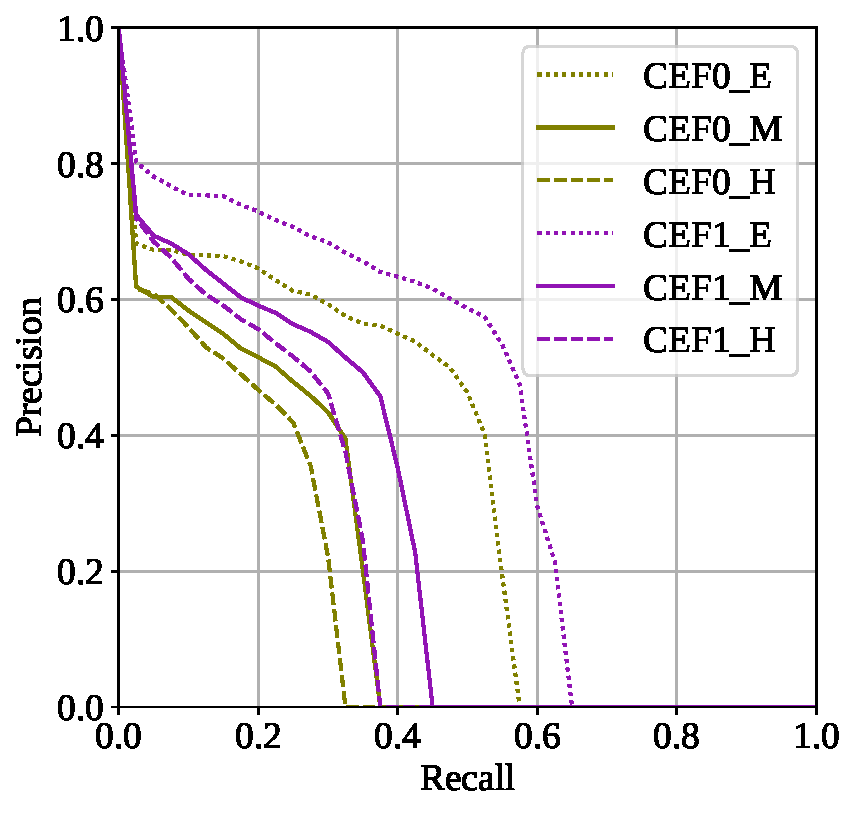
\includegraphics[width=0.4\linewidth]{../media/fpnet_pr2_cef01.pdf}}
	\caption{Precision-recall graphs for both CEF\_r0 and CEF\_r1, with lidar-based result BEF also shown for reference. In (a), the improvement between r0 and r1 manifests in an $AP_M$ increase of 5 percentage points, and at ``Easy" difficulty, the best curve in (b) has an AP of 42.57.}
	\label{fpnet_pr2}
\end{figure}

\subsection{Experiment 3: Stereo-Based Performance, using Object Detection Dataset}
Upon reviewing the most closely related paper, by \cite{wang_pseudo-lidar_2019}, the suggestion of changing the training dataset for PSMnet was taken. A pretrained stereo model was once again taken, directly from the authors, and finetuned exclusively on the same training split used by FPnet. This is in contrast to the original KITTI stereo dataset, used by the authors. The reasons for this are given below as well as further clarified in Appendix \ref{appendix_kitti}.

\subsubsection{Similarity of Ground Truths Across Datasets}
After the initial evaluation, the network was prepared and trained on KITTI data. The original authors of PSMnet provide a model pre-trained on the Freiburg SceneFlow dataset; this model was also used. After this step, however, it must be clarified that there are images in the KITTI stereo dataset that overlap greatly in similarity to those in the KITTI object detection dataset. The difference between the two datasets are essentially that one has been optimized for object detection, and the other for stereo disparity map estimation. This similarity was also noted in \cite{wang_pseudo-lidar_2019}, and this paper took the same approach to make corrections, as described below. Figure \ref{similarity_stereo_objdet} below also demonstrates the similarity between two sample images, which points to the risk of having a part of the network trained on what may be validation or even evaluation data. This would result in data leakage and thus put the validity of the results into question.

\begin{figure}[ht]
	\centering
	\subfigure[000132\_10 from Stereo]{
		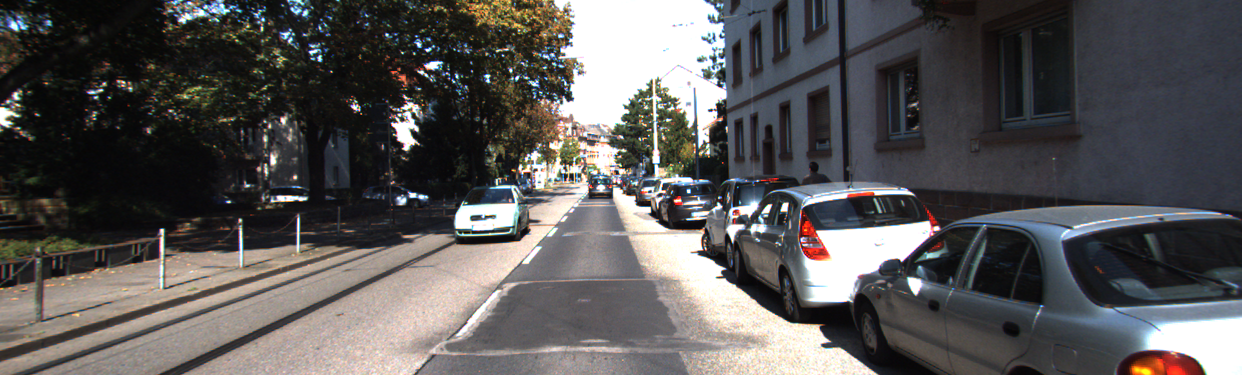
\includegraphics[width=1\linewidth]{../media/similar_000132_10_stereo.png}}
	\subfigure[000286 from ObjDet]{
		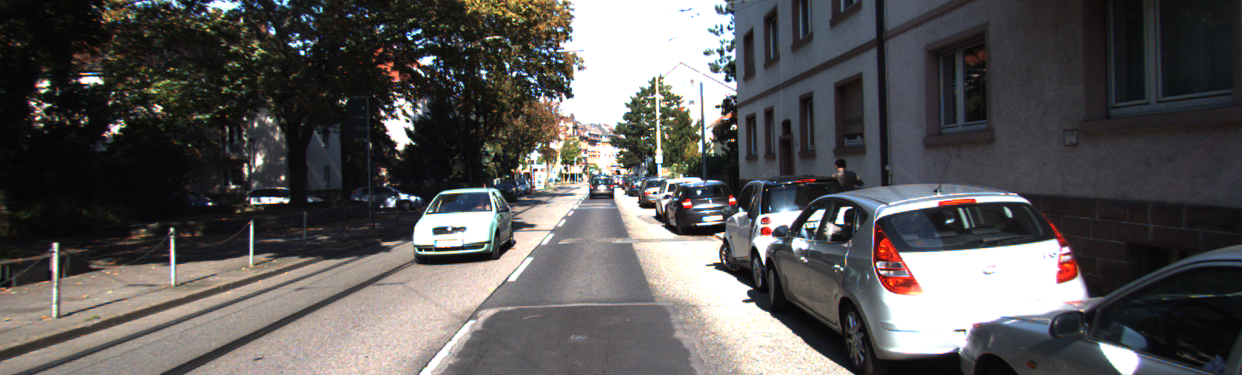
\includegraphics[width=1\linewidth]{../media/similar_000286_objdet.png}}
	\caption{Example of how two unique records from the separate datasets have overly-similar scenes. There are multiple examples of this, which creates the motivation to generate a secondary set of disparity ground truths for the object detection dataset}
	\label{similarity_stereo_objdet}
\end{figure}

In order to deal with the dataset overlap, the KITTI object detection dataset was adapted to be used for training stereo data. Lidar data was projected onto the LHS image plane, converted to integer values, then multiplied by a constant. These steps are in line with both the way that \cite{wang_pseudo-lidar_2019} were able to generate their self-made stereo ground truths as well as how the KITTI dataset authors generated their ground truth, as described in the stereo development kit. Locations in the image that have no lidar data are left alone at a value of 0.0, and finally the resulting array is saved to a PNG image file format containing integer values. Please refer to the generation script in the repository for the exact steps used to generate the pseudo ground truth stereo images.

\subsubsection{Results of Modification}
It was discovered at some point that the training / validation data used in the KITTI stereo image set was overlapping too much with images used in the KITTI object detection task. Thus, \cite{wang_pseudo-lidar_2019} was referred to and guided the change in retraining PSMnet. The difference in training is shown below.

Figure \ref{psmnet_star_train_info} below shows the loss throughout the training of PSMnet on the object detection dataset, also known as PSMstar (based on the similar name given in Wang et al's paper), as well as the original stereo dataset model for reference. 

\begin{figure}[ht]
	\centering
	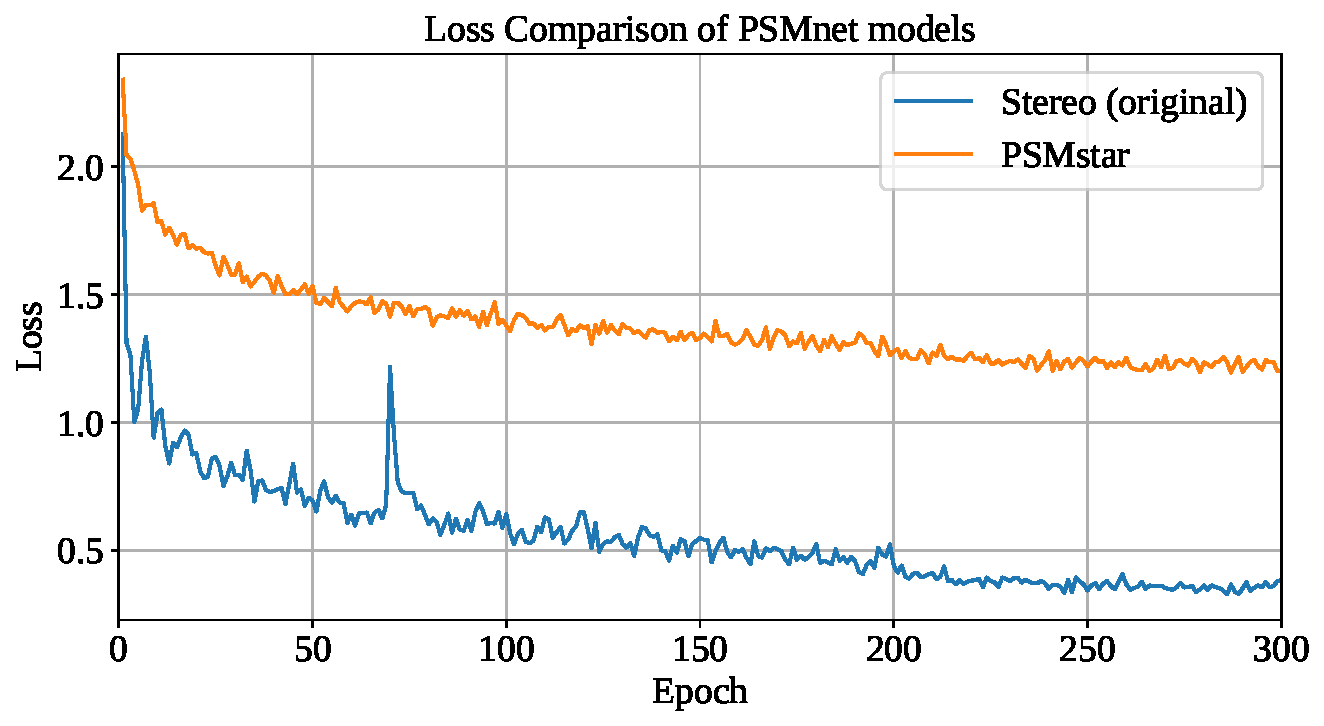
\includegraphics[width=0.7\linewidth]{../media/info_psmnet_comparison_Loss.pdf}
	\caption{Loss graphs for both the original stereo-dataset PSMnet model and the retrained, object-detection-based ``PSMstar" model. The average difference between the two curves is a loss of about 0.82. The higher loss for PSMstar may result from using self-made ground truth labels rather than using the more detailed stereo dataset versions.}
	\label{psmnet_star_train_info}
\end{figure}

In addition to the quantitative difference in training, a qualitative difference in the estimation pattern may be seen below, in Figure \ref{new_psmnet}. Overall, the change in quality may be seen as a more detailed but less contrasting depth map.

\begin{figure}[H]
	\centering
	\subfigure[Stereo estimation with original PSMnet model]{
		
\includegraphics[width=1\linewidth]{../media/ind15_psmnet_v190308_AsOf190626.png}}
	\subfigure[Stereo estimation with new PSMnet* model]{
		
\includegraphics[width=1\linewidth]{../media/ind15_psmstar_v190613_AsOf190626.png}}
	\caption{Comparison of old and new model for PSMnet. Index 15 of the KITTI Object Detection dataset. There are typically less extreme values, yet also some higher contrast in the low (distant) values, as visible by a more clear outline of two pedestrians in the center of the image. See Figure \ref{reconstruction}(a) for photo reference.}
	\label{new_psmnet}
\end{figure}


The training loss of the modified FPnet is provided below in Figure \ref{fpnet_loss3}, once again with run BEF plotted for reference. Runs CEF\_r2 and CEF\_r3 are nearly identical, although a slight modification was tested out with CEF\_r3: removing all points in the stereo-generated point cloud that were 1 meter above the sensor vertical height. However, the decrease of information, whatever its quality, seems to have had a very slight negative impact rather than positive one on the overall result.

\begin{figure}[ht]
	\centering
	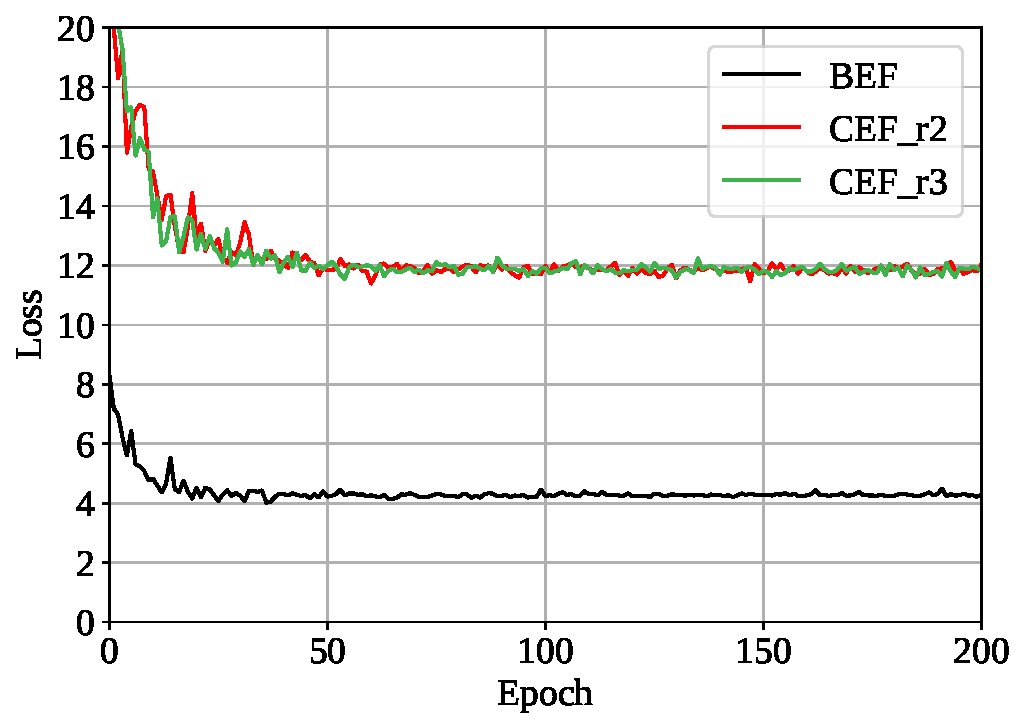
\includegraphics[width=0.6\linewidth]{../media/fpnet_loss3.pdf}
	\caption{Loss over epochs graph for Experiment 3. Run CEF\_r2 and r3 both ended training with a final loss of about 12.0. However, this value is still much higher than the reference BEF training loss.}
	\label{fpnet_loss3}
\end{figure}


The precision-recall curves for the ``Car" class is given below in Figure \ref{fpnet_pr3}, including one only for CEF\_r3, as well as the AP scores for the various difficulties in Table \ref{fpnet_ap3}.

\begin{table}[ht]
	\centering
	\caption{Experiment 3 results, with FPNet stereo-based results. Runs r2 and r3 shown across varying difficulties.}
	\begin{tabular}{|c|c|c|c|}
		\hline
		\b{Path} & \b{AP\_Easy} & \b{AP\_Med} & \b{AP\_Hard} \\ \hline
		CEF2   &    47.41     &    30.69    &    25.15       \\ \hline
		CEF3   &    45.43     &    30.45    &    24.29       \\ \hline
	\end{tabular}
	\label{fpnet_ap3}
\end{table}

\begin{figure}[H]
	\centering
	\subfigure[]{
		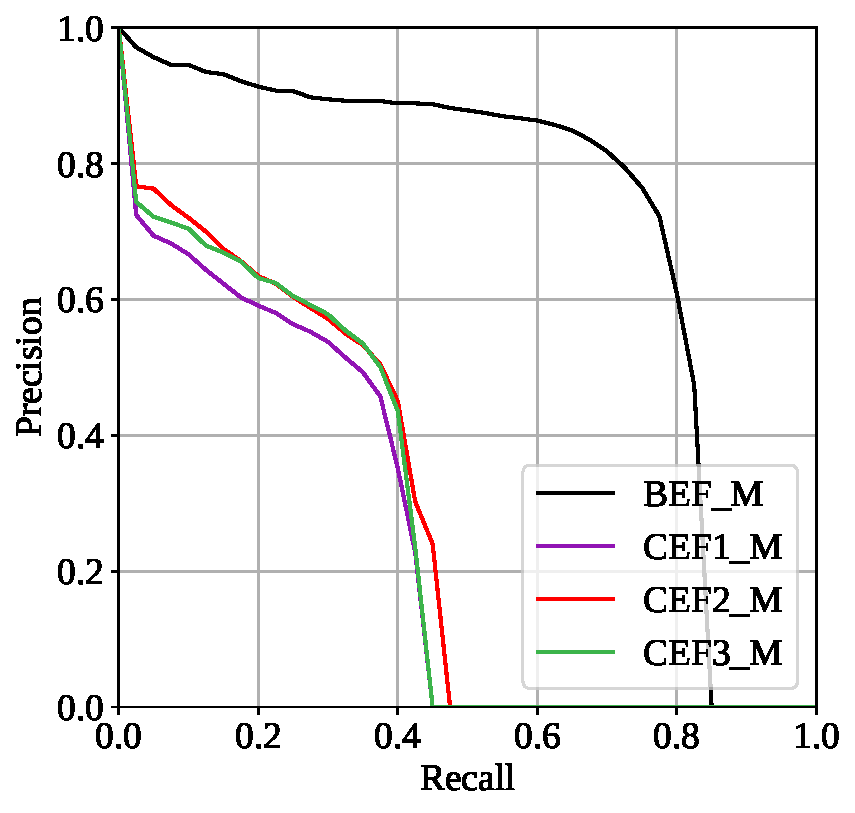
\includegraphics[width=0.4\linewidth]{../media/fpnet_pr3_multi.pdf}}
	\subfigure[]{
		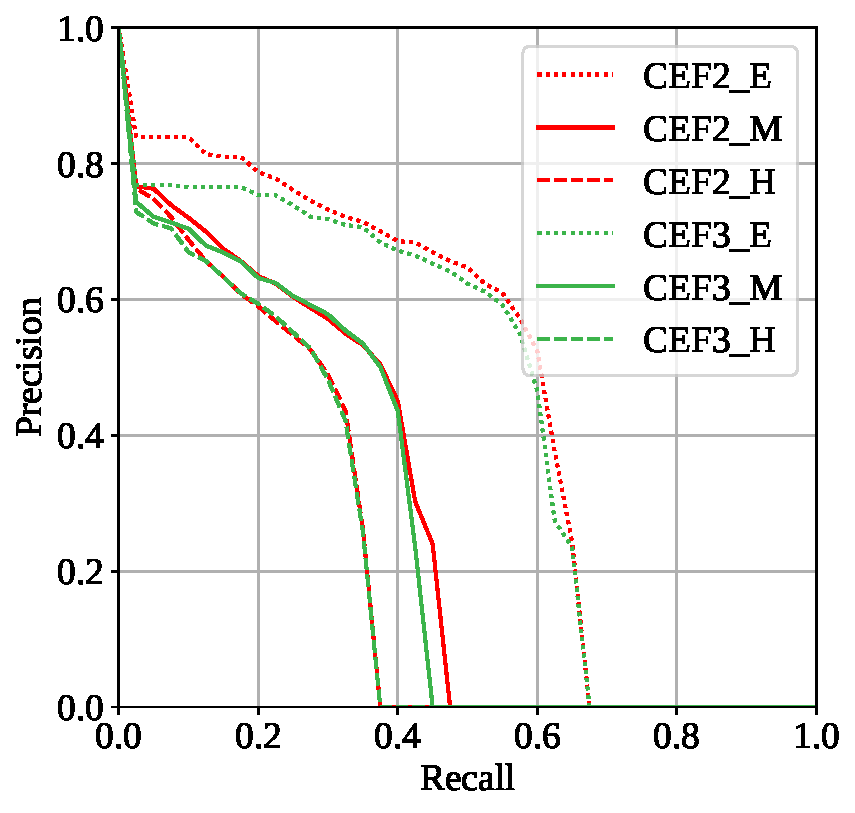
\includegraphics[width=0.4\linewidth]{../media/fpnet_pr3_cef23.pdf}}
	\caption{Precision-recall graphs for both CEF\_r2 and CEF\_r3 in (a), with lidar-based result BEF also shown for reference. Subfigure (b) further shows both across the Easy, Moderate, and Hard difficulties.}
	\label{fpnet_pr3}
\end{figure}

Although the results still lag behind lidar-based performance, Table \ref{fpnet_ap3} shows yet another improvement in AP from CEF\_r1 to CEF\_r2, improving by about 5 percentage points on ``Easy", 2 points on ``Medium", and 1 point on ``Hard".


\subsection{Comparison with Other Networks} 
In addition to both developing and testing ``SPCLnet", the official performance data of other networks was downloaded, graphed, and compared. In addition to the self-made network, the following networks were compared: 
\begin{itemize}
	\item Pseudo-Point Cloud network, by \cite{wang_pseudo-lidar_2019}
	\item STD: Sparse-to-Dense 3D Object Detector for Point Cloud, \cite{yang2019std}
	\item RCNN Stereo Network, by \cite{li_stereo_2019}
	\item RT3D: Real-time 3D vehicle detection, by \cite{zeng2018rt3d}
\end{itemize}

\begin{table}[ht]
	\centering
	\caption{Results achieved by other notable networks on the KITTI dataset.}
	\begin{tabular}{|c|c|c|c|}
		\hline
		\b{Path} & \b{AP\_Easy} & \b{AP\_Med} & \b{AP\_Hard} \\ \hline
		  STD    &    86.61     &    77.63    &    76.06     \\ \hline
		  WANG   &    55.40     &    37.17    &    31.37     \\ \hline
		  RCNN   &    49.23     &    34.05    &    28.39     \\ \hline
		  RT3D   &    28.50     &    24.10    &    20.32     \\ \hline
	\end{tabular}
	\label{fpnet_ap4}
\end{table}

\begin{figure}[H]
	\centering
	\subfigure[]{
		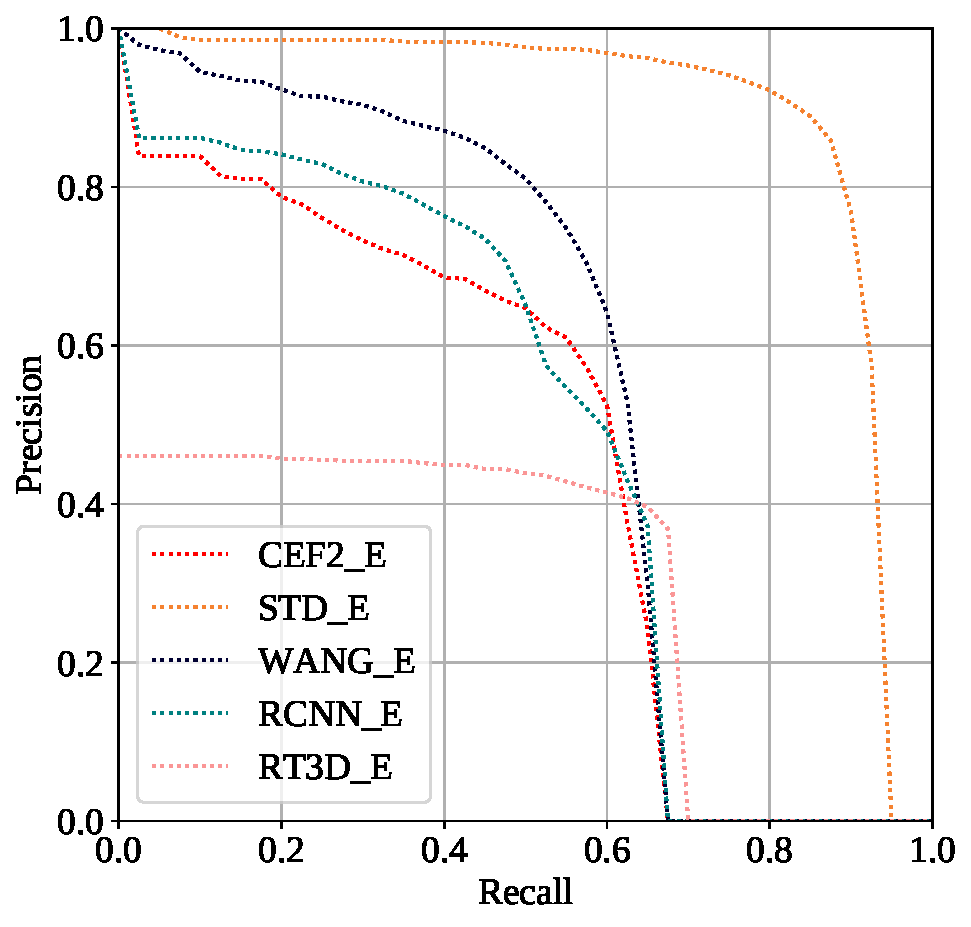
\includegraphics[width=0.487\linewidth]{../media/fpnet_pr4_multi_e.pdf}}
	\subfigure[]{
		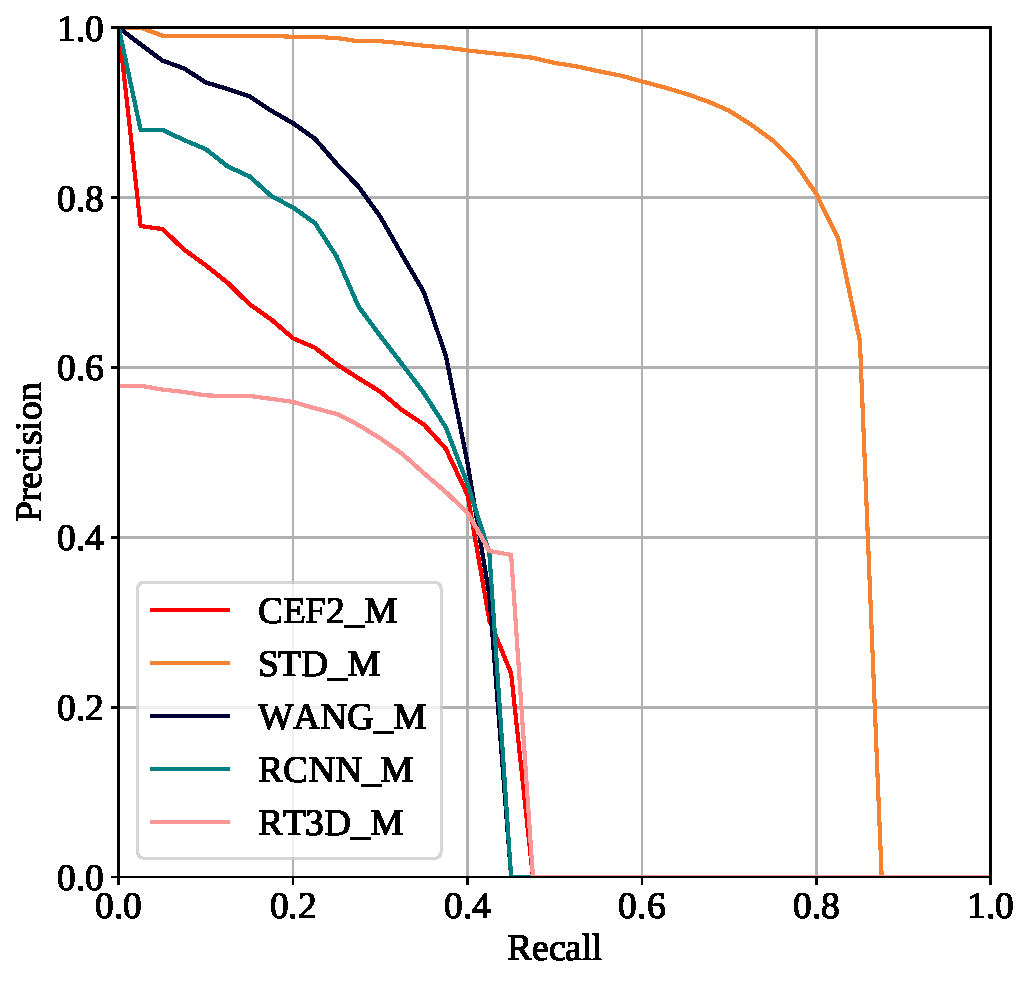
\includegraphics[width=0.487\linewidth]{../media/fpnet_pr4_multi_m.pdf}}
	\caption{Precision-recall graphs. Subfigure (a) compares run CEF\_r2 to other notable networks at Easy  difficulty. Subfigure (b) compares the same set at Moderate difficulty.}
	\label{fpnet_pr4}
\end{figure}

The best performing iteration of SPCLnet, CEF\_r2, while not performing the outright best, shares some interesting characteristics with the other stereo networks. For one, there is a sharp decline at the top-left of the curve, a trait that the RCNN curve also shares. This is typically caused when the threshold to determine outcomes is higher, occurring at higher precision and lower recall values. Next, all of the stereo algorithms reach 0.0 precision before 0.5 recall. This would indicate that even when the threshold is nearly nonexistent, there simply aren't enough valid detections to outweigh the number of False Negatives. 

% NEWSECTION ===================================================================
\newpage
\section{Conclusions and Future Work}
\label{sect_conclusions}
%1. there is potential to make a real-time system
%2. in the short range, stereo vision does perform closer to lidar, with potential to be at least a supporting sensor. 
%3. the quality of a point cloud primarily dependent on both the quality of the data as well as the quality of the neural networks trained to generate it. 
%4. This sensor has great potential in the service robot industry, where short-medium range perception is needed, with the bonus of being a passive sensor, capable of working outdoors, and 

The primary conclusion of this paper has found that stereo data indeed has great potential to compete with or extend the capabilities of a lidar based detection system. There are large strides being made in the field, from pure stereo approaches (\cite{zeng2018rt3d}, \cite{li_stereo_2019}) to macro-networks that draw inspiration from lidar based approaches (\cite{wang_pseudo-lidar_2019}). Throughout the duration of this paper's writing, there have already been a few new submissions to the KITTI dataset, indicating a growing interest in this subfield. Additionally, the KITTI dataset itself is already beginning to show its age, given that the image data itself is now nearly 7 years old since its initial publishing \cite{geiger_are_2012}, as well as the apparent need to generate one's own set of ground truth data from the object detection dataset in order to even train a stereo network on it. New datasets are showing some level of promise, such as the Apolloscape dataset \cite{huang_apolloscape_2018} or even moderately aged datasets such as \cite{cordts_cityscapes_2016}.

This paper also finds that system setup is key to stereo vision performance. Minor inaccuracies at even a few pixels can degrade system performance, and thus more investigation is needed into generating the most accurate disparity map and subsequent point cloud possible. Clearly, the latter half of SPCLnet and the pseudo-point cloud network by \cite{wang_pseudo-lidar_2019}, Frustum Pointnets by \cite{qi_frustum_2017}, can achieve near state-of-the-art results when given the right information, i.e. accurate point cloud. This indicates that both an improvement in the stereo pipeline is needed as well as an improvement on the data itself, as mentioned above.

The final conclusion of this paper is that a real-time may indeed be within reach, and the crux of achieving this real-time system is to unify and streamline the training process between disparity estimation and and point cloud manipulation. 







% BIBLIOGRAPHY =============================================

\nocite{*} % list all references
%\cleardoublepage
\bibliographystyle{apalike}
\bibliography{../refs_190521}

% kjgnote: not sure if will need the below, have simply commented it out.
%\fancyhead[RO,LE]{References}
%\listoffigures
%\listoftables
%\fancyhead[RO,LE]{Listings}
%\listofalgorithms
%\cleardoublepage


% APPENDICES ===============================================
\newpage
\appendix % change how sections are numbered
F% PERFORMANCE METRICS ==========================================================
\section{Performance Metrics}
\label{appendix_metrics}

Examples are given below for explicitly calculating the performance metrics used in determining the quality of 3D bounding box (``bbox") predictions generated by the Stereo Point Cloud network (SPCLnet)

\subsection{Intersection Over Union}
Recall that IOU is critical in vision networks for determining whether a result is a true positive (TP) or a false positive (FP). To assist in understanding IOU, a code snippet as well as an example are presented. All aspects of calculating the IOU (including area and intersection) are broken up into multiple pieces, but presented together below. For n-dimensions, the code (presented here in python) is as follows:

\begin{figure}[ht]
\setstretch{0.84} % want code to be nice and compact
\begin{lstlisting}
import numpy as np
def extent(box,inclusive=False):
    o = 1 if(inclusive) else 0 # add '1' if inclusive is true
    b = np.array(box).reshape((2,-1)).T # now in internal convention
    return np.product([i[1]-i[0]+o for i in b])
def intersection(box1,box2,inclusive=False):
    o = 1 if(inclusive) else 0 # add '1' if inclusive is true
    b1=np.array(box1).reshape((2,-1)).T
    b2=np.array(box2).reshape((2,-1)).T # internal convention
    c=np.stack((b1,b2),2)
    # for each dimension, get (min(upperbound)-max(lowerbound)) and get product
    val=1
    for i in range(len(b1)):
        ans=np.min(c[i,1,:])-np.max(c[i,0,:])
        val*=max(ans,0) # if have negative dimension, have no intersection
    return val

def IOU(b1,b2,inclusive=False,criterion=-1):
    inter = intersection(b1,b2,inclusive)
    union = extent(b1,inclusive)+extent(b2,inclusive)-inter
    if(criterion==-1):
        return inter / union
    elif(criterion==0):
        return inter / extent(b1,inclusive)
    else:
        return inter / extent(b2,inclusive)

\end{lstlisting}
\onehalfspacing % set line spacing back to normal
\caption{Python implementation of generalized IOU calculation.}
\label{code_iou}
\end{figure}

\subsubsection{Example: IOU of a Ground Truth and Prediction Label}
\def \pxpx {\ [px^2]}
\def \Asub #1{A\textsubscript{#1}}

Suppose there is an image, as given below, where there is a ground truth label `gt' and a prediction label `pr' with 2D bounding boxes formatted as \texttt{[x1,y1,x2,y2]}, all units in pixels. To determine the IOU of the image, the calculations are listed below. Because boxes represent pixel values, remember to add ``1" to each dimension.

\begin{enumerate}\itemsep=-0.5em
    \item Find area of each bounding box: \\ $\Asub{gt} = (x2-x1+1)*(y2-y1+1) = 16,335 \pxpx $ , $ \Asub{pr} = 12905 \pxpx $
    \item Find overlapping area, e.g. intersection (see \ref{code_iou} for more info): $I = 11455 \pxpx $
    \item Calculate IOU: $\frac{I}{\Asub{gt} + \Asub{pr} - I} = 0.644 $
\end{enumerate}

\begin{figure}[H]
    \centering
    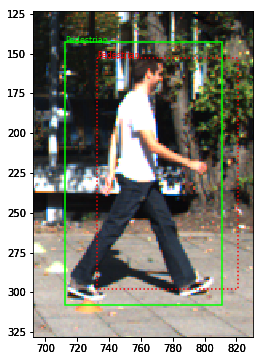
\includegraphics[width=.4\textwidth]{../media/iou_example.png}
    \caption{IOU calculation example. Ground truth (green solid) has BB: [712,143,810,307]. Prediction (red dotted) has BB: [732,153,820,297]. IOU is 0.644.}
    \label{iou_example}
\end{figure}


\subsection{Precision \& Recall}
Gathering all predictions together, one may then take the confidence score and outcome (TP, FP) of each prediction and create a precision-recall curve. To avoid extra steps regarding calculating a set of bounding boxes and determining IOU score, the following example uses a set of randomly generated outcomes values and confidence scores, listed below in Table \ref{precrecdat}.

\begin{table}[ht]
\centering
\caption{Precision-recall dummy data. Outcomes are either TP or FP, given as a `1' or `0', respectively. Confidence values are how confident the ``detection" was. In the true evaluation code, TP/FP is determined internally, and confidence values are the ``scores" in each detection label. Rows are conveniently given in order of descending confidence score.}
\footnotesize 
\begin{tabular}{|c|c|}%
\hline
\bfseries Outcomes & \bfseries Confidence % specify table head
\csvreader[head to column names]{../media/precrecdat.csv}{}% use head of csv as column names
{\\\hline\csvcoli&\csvcolii}% specify your columns here
\\\hline
\end{tabular}
\label{precrecdat}
\end{table}

The steps are as follow:
\begin{enumerate}\itemsep=-0.5em
    \item Begin with a confidence score vector and a outcomes vector
    \item Sort scores and corresponding outcomes by descending score value
    \item OPTIONAL: Identify unique index locations for approximate threshold indices (done in official code, not necessary)
    \item Create ``cumulative sum" TP-vector and FP vectors
    \item Calculate precision and recall in vector form (unrefined)
    \item Refine precision vector $pr$ and and recall vector $re$ (OPTIONAL: remove indices after TP vector stops increasing)
    \item OPTIONAL: Sort by descending recall value (done in official code, not necessary)
\end{enumerate}

\textbf{{\large Step 1: Obtain data}} \\
To begin, a randomly generated set of results (outcome and confidence scores) are given in Table \ref{precrecdat}. One may imagine that this table was generated after comparing car 3D bounding boxes against a set of ground truths and ensuring the IOU value was above a minimum threshold.

\textbf{{\large Step 2: Sort data by descending confidence score}} \\
In the case of this example, the values already sorted in this manner. Care must be taken to ensure that both a given result's confidence AND outcome (True or False) are kept in the same index location.
\begin{lstlisting}[numbers=left]
indices=np.argsort(ypred)[::-1]
ypred=ypred[indices]
ytrue=ytrue[indices]
\end{lstlisting}

\textbf{{\large Step 3 (OPTIONAL): Obtain indices of unique vectors}} \\
The purpose of this is to simply avoid needless calculation later, although empirically it has been found that the final graph and corresponding AP score are either identical or nearly so. This step WILL be carried out in this example, but may be omitted. Looking at the table, and assuming zero-based indexing as is typical in Python and other programming languages, the resulting vector is: $\texttt{[0,1,2,3,4,5,6,7,8,9,10,12,13,14,15,16,17,18]}$. Notice that index 11 and 19 are missing. ADDITIONALLY, the final index must be added to ensure that the graph terminates properly. If this step is not carried out, the correct value of the vector \texttt{threshold\_idxs} is generated instead via Line 5 below. To demonstrate the difference, please refer to Figure \ref{precrec_step3} below, and note that the AP value is still identical. In the vast majority of usage, the graph does indeed look identical.
\begin{lstlisting}[numbers=left]
if(get_unique_indices):
    distinct_value_indices = np.where(np.diff(conf))[0]
    threshold_idxs = np.append(distinct_value_indices,outcomes.size-1)
else:
    threshold_idxs = np.arange(conf.size) # sequence from 0 to N-1
\end{lstlisting}

\begin{figure}[H]
    \centering
    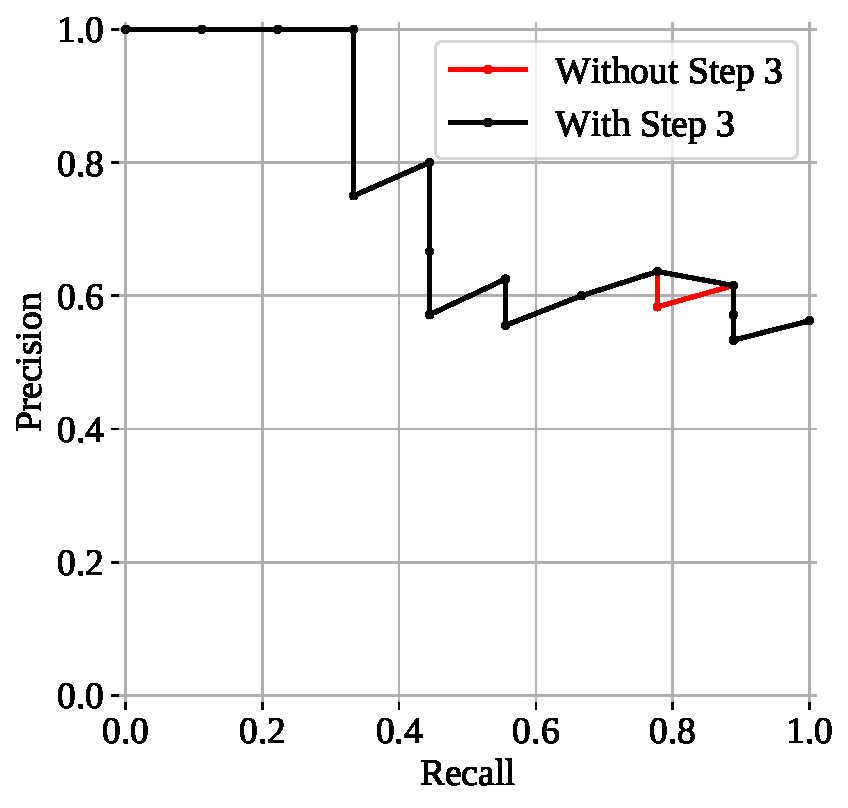
\includegraphics[width=0.45\linewidth]{../media/precrec_step3.pdf}
    \caption{Comparison of possible graph differences if Step 3 is skipped.}
    \label{precrec_step3}
\end{figure}


\textbf{{\large Step 4: Get Cumulative Sum for TP \& FP }} \\
The generation of an aggregate TP and FP vector enables precision and recall to be calculated as a vector as well, not only as scalar values. This is achieved by calculating the cumulative sum of the TP and FP arrays.
\begin{lstlisting}[numbers=left]
tps = np.cumsum(outcomes)[threshold_idxs]
fps = 1+threshold_idxs - tps
\end{lstlisting}


\textbf{{\large Step 5: Calculate Precision \& Recall}} \\
Precision and recall are calculated, but are still in a ``raw" form after this step. This means that there is some extra, unnecessary data as well as a theoretical point to be appended. As given by Equations \ref{eq_prec}, precision calculated, with some adaptation for code. Recall is often calculated differently than the theoretical form, here given as a division of the cumulative sum of true positive values by the final value.

\begin{lstlisting}[numbers=left]
precision = tps/(tps+fps)
precision[np.isnan(precision)]=0
recall = tps/tps[-1]
\end{lstlisting}


\textbf{{\large Step 6: Refine the data}} \\
Here, indices are removed after the cumulative sum of TP ceases to increase; additionally, artificial point at recall=0, precision=1 is added to the vectors (inserted at index 0). The first modification is optional, merely an aesthetic / time-saving choice, shown below in Figure \ref{precrec_step6}, but the artificial point is necessary for an accurate calculation of AP.

\begin{lstlisting}[numbers=left]
if(remove_extra_indices):
    lastind = tps.searchsorted(tps[-1])+1
else:
    lastind = -1
recall = np.append(0,recall[:lastind])
precision = np.append(1,precision[:lastind])
\end{lstlisting}

\begin{figure}[H]
    \centering
    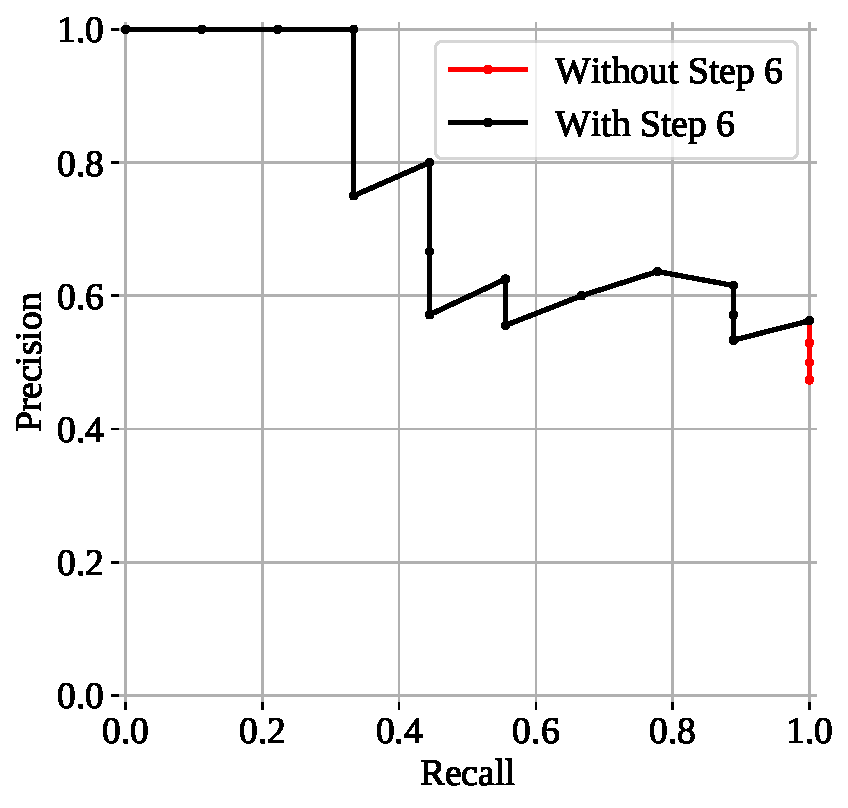
\includegraphics[width=0.45\linewidth]{../media/precrec_step6.pdf}
    \caption{Comparison of possible graph differences if Step 6 is skipped.}
    \label{precrec_step6}
\end{figure}

\textbf{{\large Step 7 (OPTIONAL): Sort by Descending Recall Value}} \\
This is an arbitrary step completed by the official matplotlib code, but may be carried out nonetheless if a certain convention is to be followed. It must be noted, however, that the proper calculation of AP requires the precision and recall vectors to be ordered by \textit{ascending} recall value.

\begin{lstlisting}[numbers=left]
recall=recall[::-1]
precision=precision[::-1]
\end{lstlisting}

Thus, the final values of precision and recall are calculated as given below in Table \ref{precrec_ans} and graphed in Figure \ref{precrec_steps}

\begin{figure}[H]
    \centering
    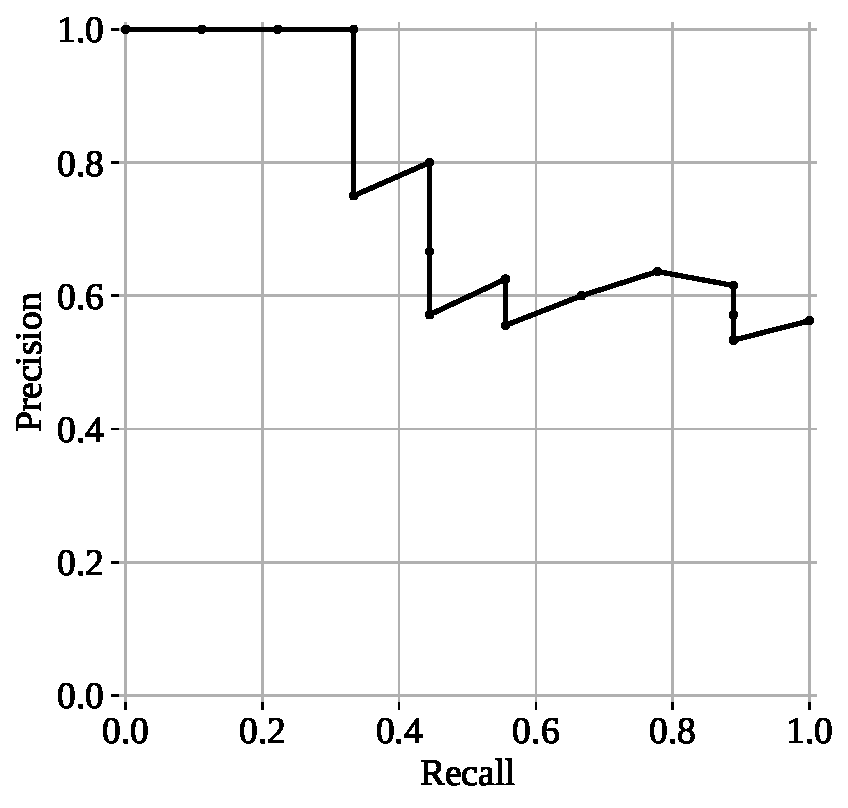
\includegraphics[width=0.4\linewidth]{../media/precrec_steps.pdf}
    \caption{Precision-recall curve if all steps are followed. Mathematically, AP value is same as without optional steps.}
    \label{precrec_steps}
\end{figure}

\begin{table}[H]
\centering
\caption{Precision-recall results, following all steps.}
\footnotesize 
\begin{tabular}{|c|c|}%
\hline
\bfseries Recall & \bfseries Precision % specify table head
\csvreader[head to column names]{../media/precrec_ans.csv}{}% use head of csv as column names
{\\\hline\csvcoli&\csvcolii}% specify your columns here
\\\hline
\end{tabular}
\label{precrec_ans}
\end{table}

\subsection{Calculating Average Precision}
To obtain the Average Precision from the previous example, simply follow Equation \ref{eq_ap}, or as implemented below (in a non-vectorized form). The AP of the values in Table \ref{precrec_ans} is 0.75992.

\begin{lstlisting}[numbers=left]
apsum=0
for i in range(0,len(precision)-1):
    print(i,end=' ')
    apsum+=(recall[i+1]-recall[i])*precision[i+1]
\end{lstlisting}






% ABOUT THE KITTI DATASET ======================================================
\newpage
\section{About the KITTI Dataset}
\label{appendix_kitti}

\subsection{Introduction}
To better understand the actual data that is being worked on, the KITTI dataset will be explained in-depth here. The acronym KITTI is a combination of ``KIT" (Karlsruhe Institute of Technology) and ``TTI" (Toyota Technical Institute, Chicago), the two cooperating institutions on the project. The very first thing to know about the KITTI dataset is that it is actually a set of datasets, each dataset specialized for some specific AI task. This means that there are some number of evaluation tasks / benchmarks, and a not-necessarily-unique dataset is used to enable completion of that task. The individual tasks are listed below with a brief description:

\begin{itemize}\itemsep=-0.5em
    \item Stereo, Optical Flow, Sceneflow (2012 \& 2015): An older (2012) and updated (2015) task comprised of 200 training and 200 test scenes. Each scene consists of a left and right image as well as a ``multi-view extension".
    \item Depth Completion / Estimation: A task comprised of about 93 thousand scenes containing RGB images and lidar scans.
    \item Visual Odometry / SLAM: 11 training and 11 testing stereo sequences with relevant grayscale, color, lidar, and ground truth poses.
    \item 2D / 3D / Bird's Eye View (BEV) Detection: 7481 training and 7518 test scenes with relevant color images, temporally preceding images, and lidar
    \item Single-/Multi- Object Tracking: An older (single) and in-development (multi) task consisting of multiple training and test sequences with relevant image, lidar, and GPS/IMU data.
    \item Road / Lane Detection: Around 289 training and 290 test images used for detecting various road scenes, containing image and lidar information.
    \item Semantic / Instance Segmentation: A task comprised of a set of stereo images like the Stereo task, but containing pixel-level localization of each class.
\end{itemize}

Each evaluation task also brings with it a ``dev kit" (a set of files that explain some of the technical information as well as helpful code), relevant camera / sensor calibration data of some kind, as well as some kind of ground truth label / file for each scene to assist with training. It should be noted that raw data of each dataset is available as well, but these are often unused and only kept as original source files for transparency. 

Each task is associated with one or more papers published by KIT and TTI, but these will not all be listed here. Instead, we shall now explain two datasets, especially the most relevant one: the KITTI object detection dataset, referred to as the KITTI dataset.

\subsection{The Stereo Dataset}
The stereo dataset, specifically 2015, will be briefly covered to describe its merits as well as why it presented overlap issues with the object detection dataset. What makes the stereo dataset important is that it is the dataset that was initially used to finetune the Pyramid Stereo Matching network and also the dataset used to help it achieve such a high position in the stereo benchmark.

The dataset itself is made up primarily of 200 training scenes and 200 testing scenes. The training scenes contain ground truth disparity maps, while the testing scenes do not and are used for final evaluation and submission to the benchmark website. For the project, only the training scenes were used. Each training scene is comprised of a left-hand side (LHS) color image, a RHS color image, a calibration file (containing transformation and other matrices), and a ground truth disparity file. There is also an available ``multi-view extension", containing 20 extra frames per scene, but this was not used. Figure \ref{stereo_sample} below shows all relevant data in a single sample scene: the left and right images, as well as a disparity map ground truth.

The ground truth labels were generated by a ``semi-automatic" process, as described by Menze and Geiger: the process was to ``extract disparity maps directly from the 3D information int he laser scans and fit geometrically accurate CAD models to moving 3D point clouds" \cite{menze_object_2015}. This explains several things about the ground truth disparity map in Figure \ref{stereo_sample}(c): the image is generally sparse, has no sample values above a certain horizontal line, and has a high density of pixels in the region where a car is outlined.

\begin{figure}[H]
    \centering
    \subfigure[left image]{
        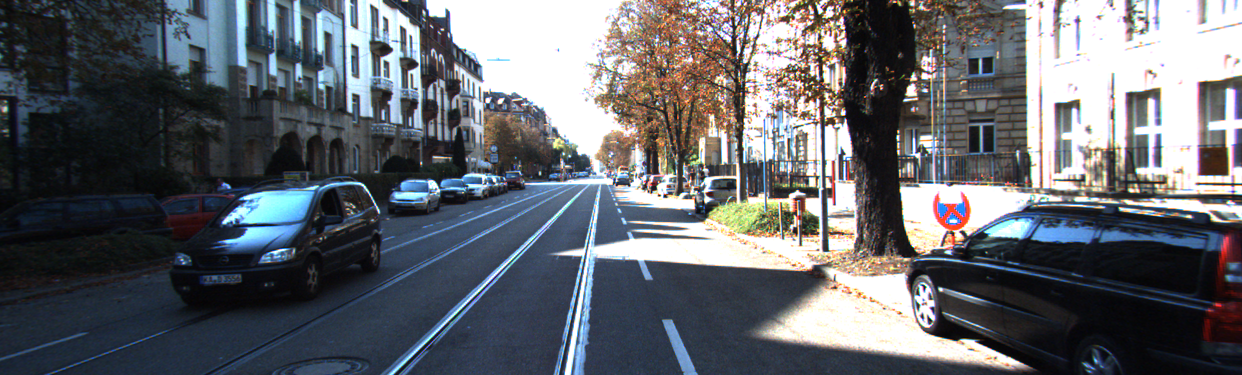
\includegraphics[width=0.487\linewidth]{../media/stereo_LHS_000000_10.png}}
    \subfigure[right image]{
        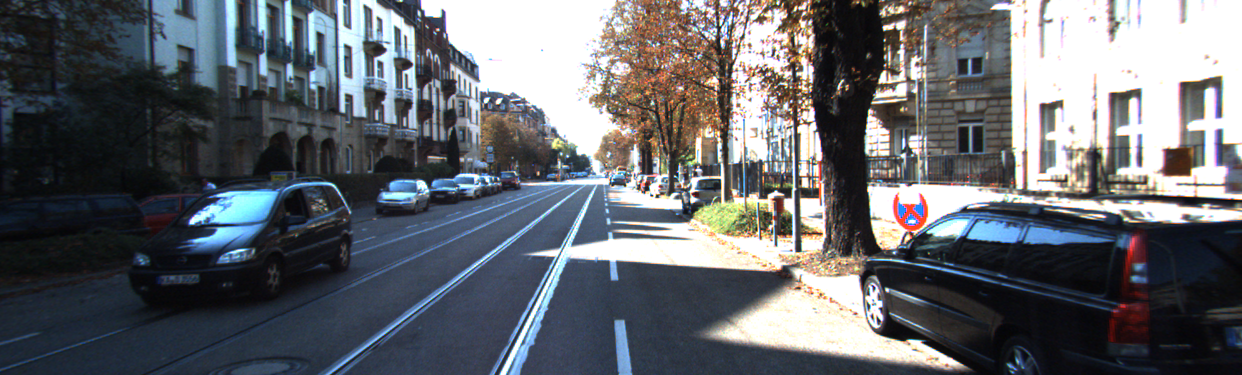
\includegraphics[width=0.487\linewidth]{../media/stereo_RHS_000000_10.png}}
    \subfigure[Ground truth disparity map. The value range for the original ground truth file may lie anywhere in the range of 1 to about 33,000.]{
        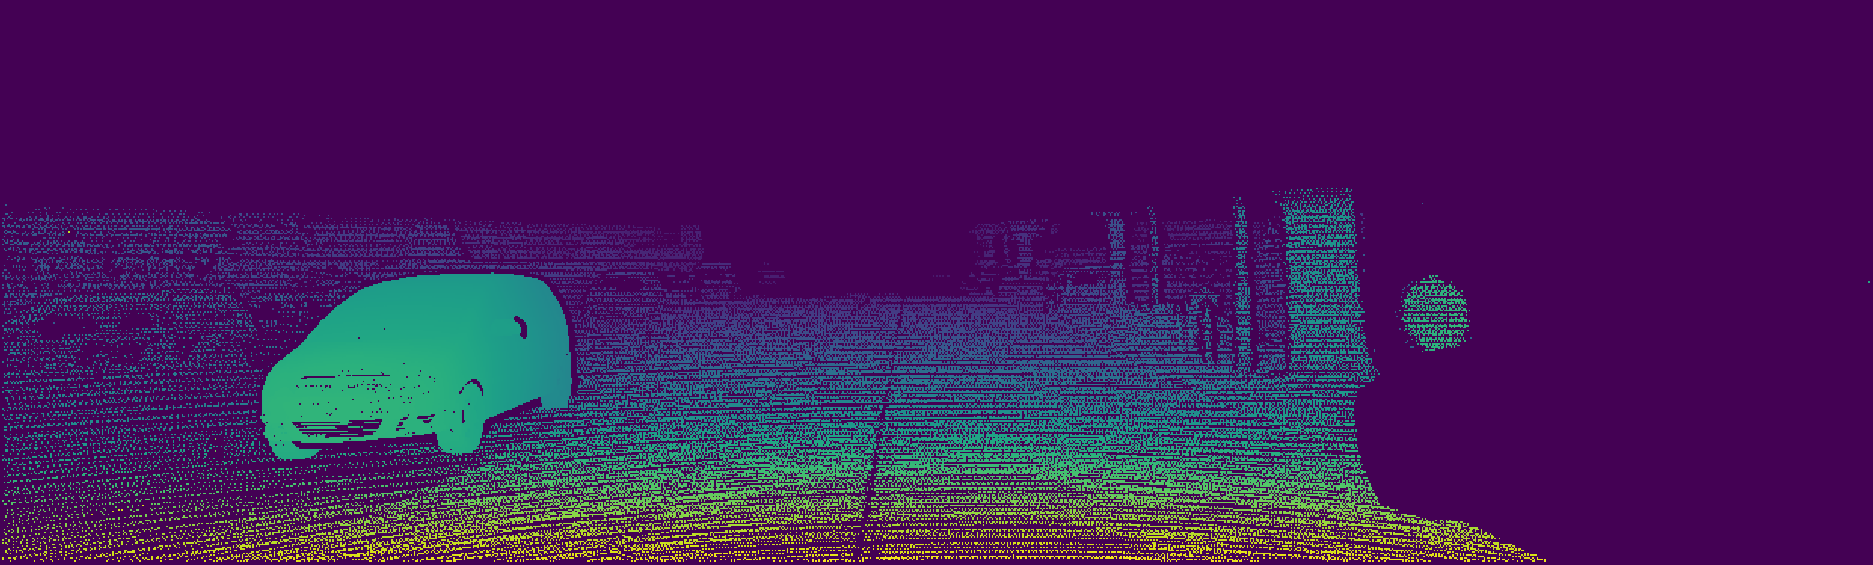
\includegraphics[width=1\linewidth]{../media/stereo_GTdisp_000000_10.png}}
    \caption{Sample scene. Index 000000\_10 of the KITTI stereo dataset.}
    \label{stereo_sample}
\end{figure}



Ultimately, however, this dataset was not used for the primary reason described by \cite{wang_pseudo-lidar_2019}: there was an unacceptable amount of overlap between the stereo dataset training data and the similar but unrelated object detection dataset. This could lead to validation images being used in training, an issue known as data leakage. Figure \ref{similarity_stereo_objdet}, shown in Section 3, gives an example of a scene in the stereo dataset nearly matches a scene in the object detection dataset.

\subsection{The Object Detection Dataset \& Statistics}
The Object Detection dataset is the primary source of sensor data and media for this project, including PSMnet once it was determined that the stereo dataset had too much similarity with this dataset. This similarity could lead to data leakage, contaminating the integrity of the results. The Object Detection dataset is comprised of 7481 training scenes and 7518 testing scenes. The testing scenes were ignored for the purposes of this project, since they are unlabeled for KITTI benchmarking. Each scene in the training dataset contains a LHS (left-hand side) image, RHS image, lidar data, calibration data, and ground truth labels. An example of the images and lidar are given below in Figure \ref{objdet_sample}.

\begin{figure}[H]
    \centering
    \subfigure[LHS image]{
        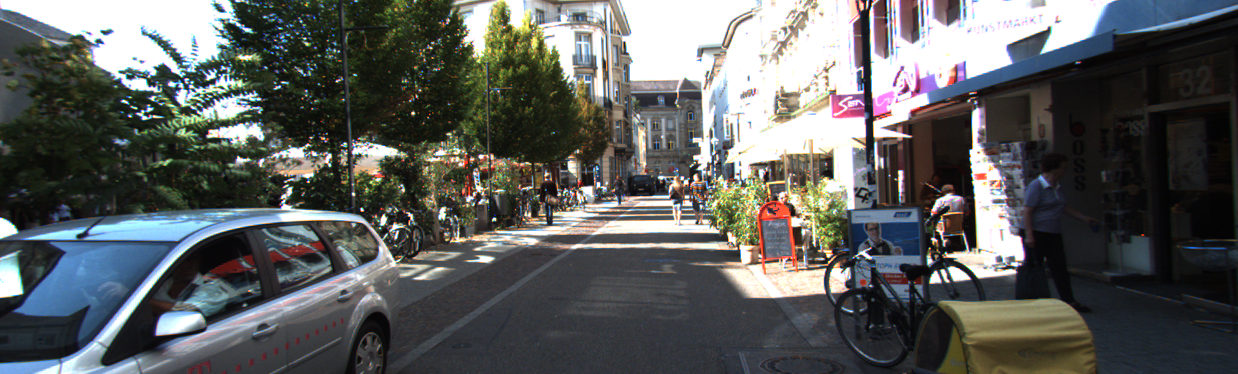
\includegraphics[width=0.487\linewidth]{../media/objdet_LHS_000015.png}}
    \subfigure[RHS image]{
        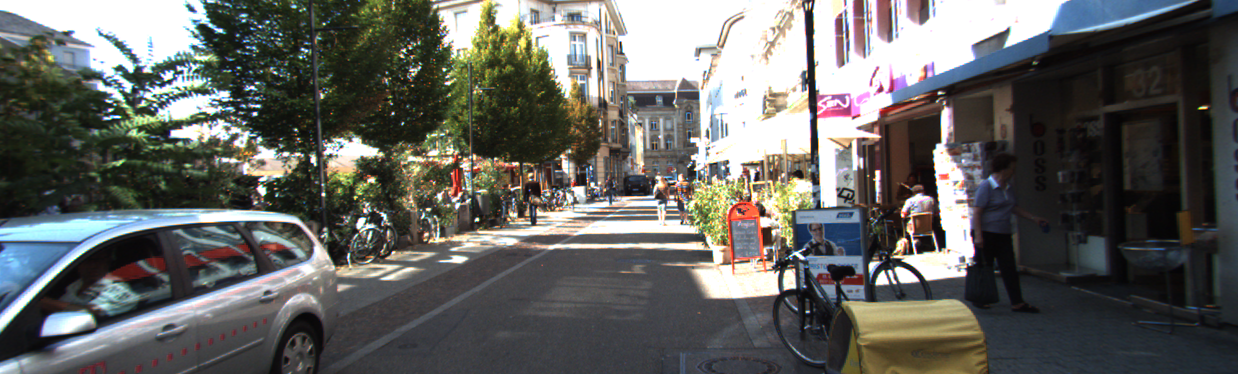
\includegraphics[width=0.487\linewidth]{../media/objdet_RHS_000015.png}}
    \subfigure[Velodyne lidar points projected onto image plane. Gray background for ease of viewing. Individual points use viridis colormap.]{
        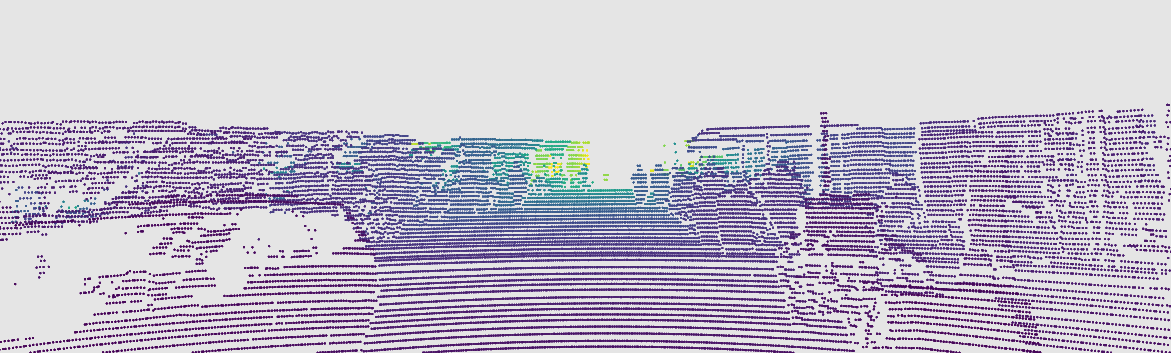
\includegraphics[width=1\linewidth]{../media/objdet_lidar_000015.png}}
    \caption{Sample scene from object detection dataset. Index 15 of the KITTI Object Detection dataset.}
    \label{objdet_sample}
\end{figure}

In addition to the above lidar projection, the point cloud may be better visualized with an isometric view, rather than one from the camera's perspective. This is provided below. As is immediately obvious in Figure \ref{objdet_lidar_sample} and from knowledge of the hardware itself, a lidar scan is capable of capturing points surrounding the sensor in a 360\deg horizontal view. However, because of the nature of a typical color camera, points that are outside the camera's field of view are filtered out.

Another key piece of the object detection dataset is the label data. Ground truth labels are simply lines of text that contain an array of information about each instance of an object in the scene. An example label with value names is given below in Table \ref{kitti_label_sample}. There are 15 values in each label, and an extra 16th ``Score" value for prediction labels, a decimal value in range [0,1]. The raw text for this label simply looks like so: \\
\texttt{Car 0.89 0 2.29 0.00 194.70 414.71 373.00 1.57 1.67 4.14 -2.75 1.70 4.10 1.72} \\

\begin{figure}[H]
    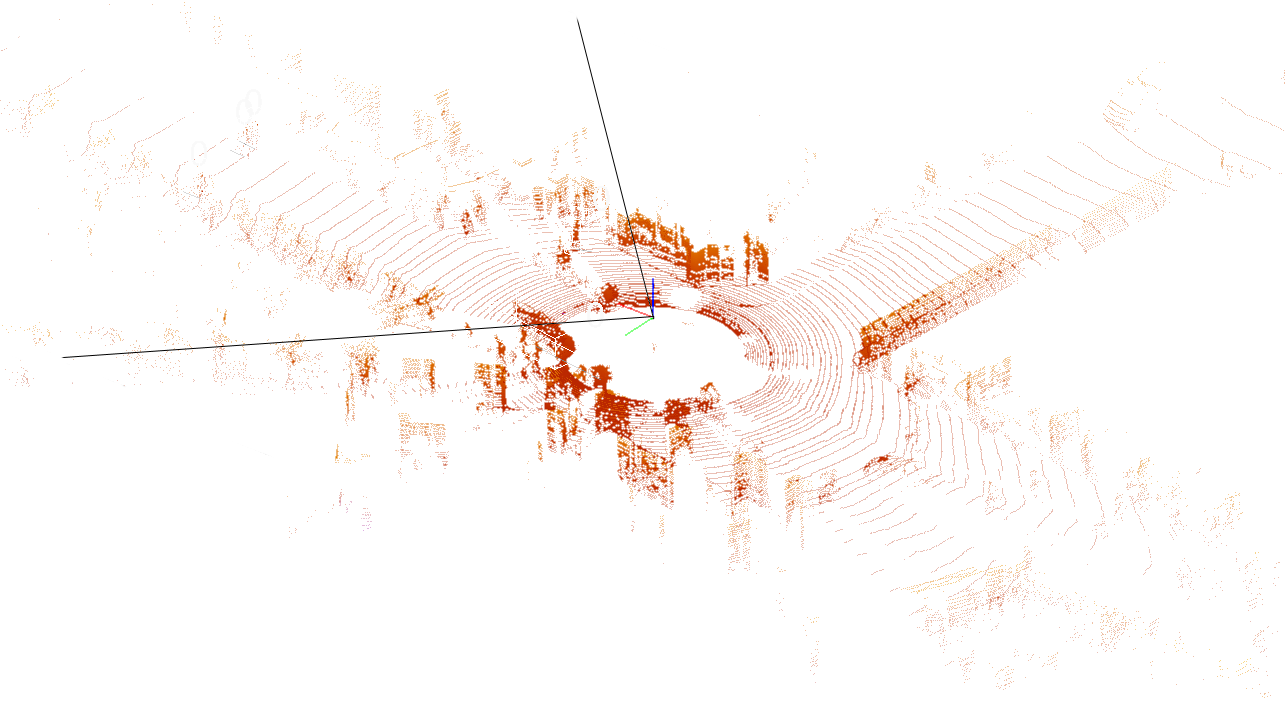
\includegraphics[width=0.8\linewidth]{../media/objdet_lidar_BEV_000015_light.png}
    \caption{Lidar pointcloud, alternate view. 3D bounding boxes are included as well as the horizontal field of view (angled lines leading away from coordinate system origin). Index 15 of the KITTI Object Detection dataset}
    \label{objdet_lidar_sample}
\end{figure}

\def \DEG{$^{\circ}$} % Don't want to import extra package for no reason right now.

\begin{table}[H]
	\centering
	\caption{KITTI object detection sample label from a given scene. Index 15 of the KITTI Object Detection dataset}
	\footnotesize
\begin{tabular}{|c|c|c|c|c|c|c|}
	\hline
	Class & Trun & Occl & Obs  & BBx1  & BBy1   & BBx2  \\
	\hline
	Car   & 0.89       & 0         & 2.29 & 0.00  & 194.70 & 414.71 \\
	\hline
\end{tabular}
\begin{tabular}{|c|c|c|c|c|c|c|c|}
	\hline
	BBy2   & HT   & WD   & DP   & Xc    & Yc   & Zc   & Roty \\
	\hline
	373.00 & 1.57 & 1.67 & 4.14 & -2.75 & 1.70 & 4.10 & 1.72 \\
	\hline
\end{tabular}
\label{kitti_label_sample}
\end{table}

In order to better understand the meaning of each value, each dataset provides a ``development kit" that contains a ``readme.txt" file. In the object detection devkit, the following text reproduced in Figure \ref{kitti_devkit_info}. Some of the names are different than what is used, but the order and purpose are identical.

\begin{figure}[ht] %h=here,t=top,b=bottom,H=exactlyHere
	\setstretch{0.8} % want code to be nice and compact
	% note: optional line numbers argument
	\small
	\begin{lstlisting}[language=tex]
Ct.  Name         Description
----------------------------------------------------------------------------
1    type         Describes the type of object: `Car', `Van', `Truck',
                      `Pedestrian', `Person_sitting', `Cyclist', `Tram',
                      `Misc' or `DontCare'
1    truncated    Float from 0 (non-truncated) to 1 (truncated), where
                      truncated refers to the object leaving image boundaries
1    occluded     Integer (0,1,2,3) indicating occlusion state:
                      0 = fully visible, 1 = partly occluded
                      2 = largely occluded, 3 = unknown
1    alpha        Observation angle of object, ranging [-pi..pi]
4    bbox         2D bounding box of object in the image (0-based index):
                      contains left, top, right, bottom pixel coordinates
3    dimensions   3D object dimensions: height, width, length (in meters)
3    location     3D object location x,y,z in camera coordinates (in meters)
1    rotation_y   Rotation ry around Y-axis in camera coordinates [-pi..pi]
1    score        Only for results: Float, indicating confidence in
                      detection, needed for p/r curves, higher is better.
	\end{lstlisting}
	\onehalfspacing % set line spacing back to normal
	\caption{Original text from readme.txt file of devkit\_object resources. The columns are: Ct. (``count"), Name (of value), and Description.}
	\label{kitti_devkit_info} % label goes last
\end{figure}

Beyond a few samples of the dataset, some statistics about the dataset can be found in both the accompanying paper as well as by looking through the dataset itself. From the original 2012 paper, \cite{geiger_are_2012} provided a subfigure of the class count across both training and validation data, reproduced below in Figure \ref{kitti_graph_objectcount}. When observing only the training data, the count of each class can be described. A quick summary of each value across all labels in the training dataset is given below in Table \ref{kitti_label_stats}. Note that the min/max range ignores the DontCare class and its values, such as -1000 for $z_c$.

\begin{figure}[H]
	\centering
	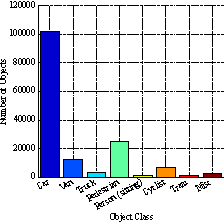
\includegraphics[width=0.4\textwidth]{../media/kitti_graph_objectcount.pdf}
	\caption{Object class count in KITTI object detection dataset, reproduced from \cite{geiger_are_2012}.}
	\label{kitti_graph_objectcount}
\end{figure}

\begin{table}[H]
	\centering
	\caption{KITTI dataset label statistics. Each numbered value's minimum and max values are given. Variables xc, yc, and zc are distance to the bounding box center of mass, and pixel values are given to sub-pixel accuracy.}
	\footnotesize
	\begin{tabular}{|c|c|c|c|c|}%
		\hline
		\bfseries Name & \bfseries DataType & \bfseries Unit & \bfseries min & \bfseries max % specify table head
		\csvreader[head to column names]{../media/kitti_label_stats.csv}{}% use head of csv as column names
		{\\\hline\csvcoli&\csvcolii&\csvcoliii&\csvcoliv&\csvcolv} % specify your columns here
		\\\hline
	\end{tabular}
	\label{kitti_label_stats}
\end{table}

The final bit of interesting statistical information may be found by counting the number of instances of each class. This is already provided by \cite{geiger_are_2012}, but in verifying the values provided only in the training data the exact number of instances of each class are listed below in Table \ref{kitti_class_stats}.

\begin{table}[H]
	\centering
	\caption{KITTI object detection class count. Semi-automatically counted through only labeled training data.}
    \footnotesize 
	\begin{tabular}{|c|c|c|c|c|c|c|c|c|}
		\hline
		Class & Car   & Pedestrian & Van  & Cyclist & Truck & Misc & Tram & Person\_sitting \\ \hline
		Count & 28742 & 4487       & 2914 & 1627    & 1094  & 973  & 511  & 222             \\ \hline
	\end{tabular}
	\label{kitti_class_stats}
\end{table}


\subsection{Evaluation Difficulty Levels}
One of the last but certainly not least important aspects of the KITTI dataset is the difficulty rating system. The KITTI dataset certainly has a variety of scenes and training data, but it also allows scoring to be performed on three difficulty levels, defined as follow:

\begin{enumerate}\itemsep=-0.6em
	\item Easy: 40 pixel min bbox height, max  level: Fully visible (0), max truncation: 15\%
	\item Moderate: 25 px minimum bbox height, max occlusion level: 1, max truncation: 30\%
	\item Hard: 25 px min bbox height, max occlusion level: 2, max truncation: 50\%
\end{enumerate}

Naturally, the ``Easy" difficulty typically earns a higher AP score than ``Moderate" (or ``Medium"), and ``Moderate" in turn typically yields a higher AP score than ``Hard". The official final score that a network receives when submitted to the KITTI Leaderboard is the ``Moderate" mean AP score. This paper specifically deals with the ``Car" class, so we may be able to better understand how these difficulties affect other parameters. Specifically related to the ``Car" class, 3D bounding box is considered a detection at 70\% overlap with a ground truth. The other two classes, ``Pedestrian" and ``Cyclist", only require an overlap of 50\%. The remaining other classes are not typically included in evaluation and scoring.

In the paper \cite{wang_pseudo-lidar_2019}, the ``Easy" evaluation for the ``Car" class is said to test on car labels located mostly within 30m of the ego vehicle, which was also claimed by another group, \cite{yang_pixor:_2018}. This was verified, and it is shown below in Figure \ref{kitti_labels_easyCar}.

\begin{figure}[H]
	\centering
	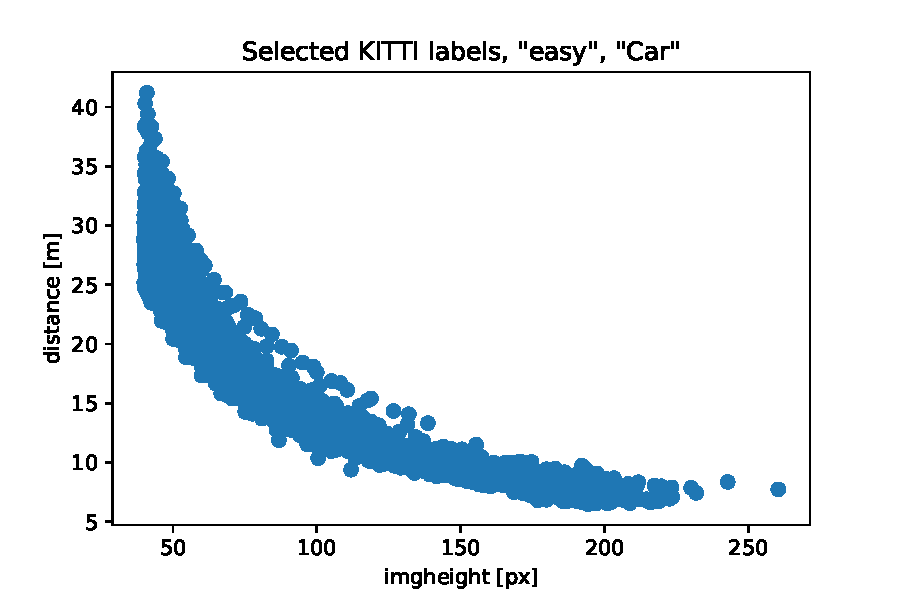
\includegraphics[width=0.6\textwidth]{../media/kitti_labels_easyCar.pdf}
	\caption{Filtered set of labeled training data containing only labels with the ``Car" class and those which are defined as ``Easy" difficulty. Just over 3\% of these filtered labels are beyond 30m. An interesting observation that may be made from the pixel height / distance relationship is that they are inversely correlated.}
	\label{kitti_labels_easyCar}
\end{figure}

% glhf



\end{document}
% END OF MAIN DOCUMENT =========================================================

at this point, can write anything you want, so go ahead and keep whatever you like in this section.

